\chapter{Visualization with Commit Data}
\label{chap:visualization}

% TODO add summary of approach
The goal of the research proposes and assess a research tool for predicting changes within a project. This is accomplished through mining of software data, analysis of collected data, candidate feature analysis. Once the data has been collected a further analysis is used to extract key features. As part of this analysis visualizations through custom visualizations. The visualizations help to provide insights into the data set. Candidate features are then selected from possible features and analyzed later on to attempt to determine the best feature set.

% TODO fix segway into this paragraph

\section{Collection}
\label{sec:collection}

% TODO verify predominate number (90%)
In order to be able to predict changes within a project some project data must first be collected. The data collection is targeted towards \gls{oss} projects that are developed using GitHub. Specifically projects were selected that are predominately written in Java. A project would be predominately written in Java if it has over $90\%$ of the source code in Java. Some of the sampled projects, especially larger ones, included other languages for small purposes such as a database schema outline. The purposed approach is not language specific in theory however in order to simplify the implementation the method was restricted to only work with Java. The data collection process simply data mines the complete development history of the project through the commits stored in GitHub. The commit data includes developers related, the source files and the changes associated with them. Finally the project's release information is collected in the form of tags is recorded.

The data is kept unprocessed and stored directly into a relational database (MySQL) that allows the data to be used and manipulated without requiring access to GitHub again.  This was ideal during the more initial phase of the research since a decoupled collection allows for various methods of analysis to be applied on the dataset without requiring the data to be download again. The collection process can take long to perform and depends largely on the size of the project. In the case of an incomplete collection can be resumed to collect the remaining data. Similarly, a project that was previously collected can be mined a second time to collect any new commits made to the project. These maintenance collections will often be much smaller and require a smaller amount of time to collect.

%<<< TODO create a table which outlines the data elements >>>
% TODO create a figure of an api return

The collection method chosen for mining data from GitHub projects was using GitHub's web \gls{api}. The GitHub \gls{api} allows access to the complete set of publicly available information stored in GitHub. Accessing the data through the web \gls{api} allows for the collection process to be automated and vastly simplifies the process. This project commit history dataset can be rather large since it includes a snapshot of the commit, all the change data and developer data related. Therefore the process may take both a long time and lots of space. The collection process requires both the name of the developer and repository. To actually collect the data from GitHub a ruby script was used. This collection is built around a Ruby library, \textit{github\_api}\footnote{\url{https://github.com/piotrmurach/github}}, which is a convenient wrapper for GitHub's web \gls{api}. The script systematically collects the desired data related from a given GitHub project to be stored locally. As noted above the collection can take a bit of time to complete since it must go commit by commit to collect the necessary data.

% TODO integrate this with above explanation of VCS and git
Some aspects of the GitHub project's dataset are not collected as they were deemed unnecessary however the collection method could easily be extended to collect the other aspects. The aspects not collected are the issues, branches, forks and pull requests. The issues data outlines the problems reported in the project by users or developers of that project. GitHub allows for issues to be optional and thus some projects do not offer issue reporting through GitHub. Branches are also directly related to the project and they are essentially different workspaces for the developers. They allow for development of different versions (such as a development version compared to a stable version). For simplicities sake the approach assumes that the main branch (the master branch) is the development branch and the target of the analysis. Therefore the branches are ignored at least for the scope of this work and could be included in future work. Of course other branches could be analyzed however the perspective of the other branches typically originates from the master branch.

A similar subset of data not collected or used for this approach is any forks of the repository. In GitHub a fork is an externally created branch of the project. The major differences between a fork and a branch are that a fork is owned by another developer and a fork is in fact a project onto itself. This allows for a developer who are not contributors to make a copy of the project and work on it without affecting the original. Forks typically denote a deviation from the original project that is unlikely to be reconciled. Finally, pull requests facilitate external developers making small changes which tend to be fixes to problems found or desired feature implementation. The owner of the original repository can then decide to integrate the changes made the original repository.


%- TODO explain a little more
%    - about using the api commands and how this is entirely automatic. Simply point to repo owner and name and it collects
%    - language agnostic for collection
%    - What is not collected:
%        - issues
%        - forks
%        - pull requests

\section{Storage}
\label{sec:storage}

As mentioned above the data is stored in a MySQL relational database which leverages \gls{sql}. There are three databases used for the collection and the analysis. The first stores the raw mined data, whereas the second stores the analyzed data in a more convenient layout to be used later. Finally, the third database stores the same data as the second however uses a different relational database implementation because of some limitations within MySQL. This third database uses PostgreSQL, which has a more advanced set of features than MySQL and is simply a clone of the second database. The specific limitations that were encountered will be discussed more fully later in this section.

\begin{figure}[!ht]
    \centering
        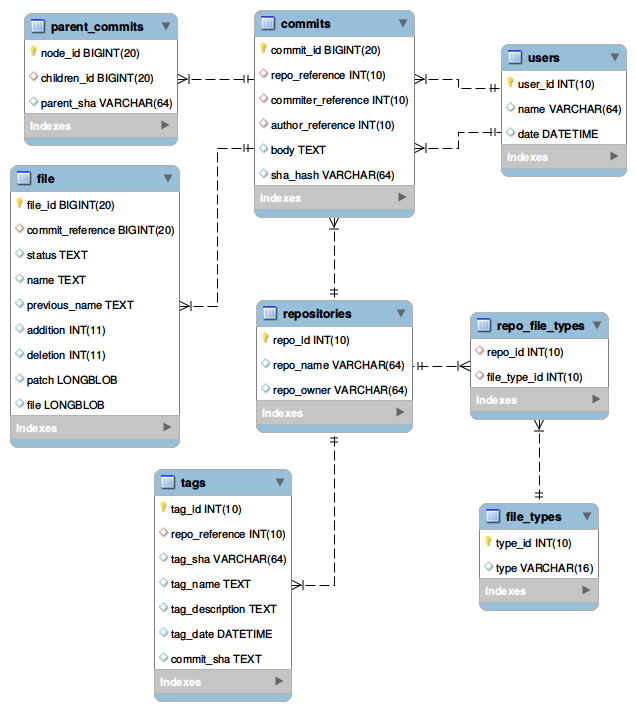
\includegraphics[width=1.0\textwidth]{images/github_data_schema}
    \caption{GitHub Data Schema}
    \label{fig:github_data_schema}
\end{figure}

%TODO re-factor this
The first database, \textit{github\_data}, stores the semi-raw data collected from GitHub's \gls{api}. This database contains 8 tables which store various aspects about the projects considered potentially important for the analysis later on. The tables of primary concern are \textit{repositories}, \textit{commits}, \textit{users}, \textit{files} and \textit{tags} tables. The complete schema is outlined in \autoref{fig:github_data_schema}. Other aspects are available from the \gls{api} and if need the database could be extended to store more elements as necessary. In some cases data from the \gls{api} is not available for one reason or another (usually inaccessible files or such) these are simply removed or a note is made of them depending on their importance. For example, files missing that already do not contain Java code are not essential and if inaccessible are ignored. If a Java file is inaccessible a note is made as this is a greater concern. These files can be retrieved if enough information is available (previous version and corresponding patch file). In the case that insufficient information is available the analysis can still be applied but will likely adversely effected the result.

After storing the data in the \textit{github\_data} database, the analysis process is done. The \textit{parsing} script is run next and discussed further in the \autoref{sec:parsing}. The results are then stored the \textit{project\_stats} database that is very similar in layout to the first database except some extra tables have been added and a few data items have been removed. Mostly the storage expansions have been to hold change information calculated from the analysis of the data. The complete schema is outlined in \autoref{fig:project_stats_schema}.

\begin{figure}[!ht]
    \centering
        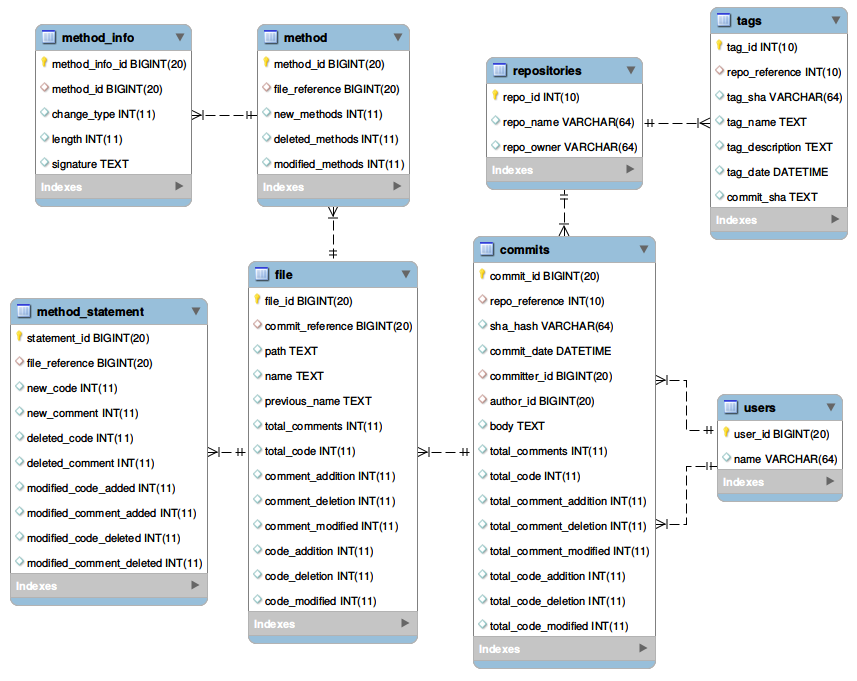
\includegraphics[width=1.0\textwidth]{images/project_stats_schema}
    \caption{Project Stats Schema}
    \label{fig:project_stats_schema}
\end{figure}

The third and final database uses PostgreSQL because of limitations within the MySQL implementation. The calculation of the candidate features, discussed in further detail in \autoref{sec:experimental_project_data}, required a more versatile partitioning function and the ability to perform multiple inner queries. The first of which is more difficult to implement and the second is not available at all MySQL. Therefore the data was transferred over to PostgreSQL, using simple program called \textit{pgloader}\footnote{\url{http://pgloader.io/}}. Only one difficulty was encountered during the transferring process. One of the tables in the MySQL database was called \textit{user}, however in PostgreSQL this is a reserved table name and therefore the table cannot be interacted with properly. The work around was to simply rename the table in MySQL prior to transferring to avoid any issues with the database. After transferring the data over to the PostgreSQL data change predictions were ready to be preformed.

\section{Parsing}
\label{sec:parsing}

The raw data collected from GitHub is stored and undergoes an analysis to extract more refined details. The process first requires the changes from a commit, the patches, to be merged into their corresponding full file. A patch is simply a stub file which summarizes the changes that occurred within a source file. Once the patch is merged with the raw source file a full file is formed that contains every change as well as the source code that did not change. Within a patch file and a full source file three different types of changes are present; additions, deletions and no change. These are represented as a plus sign, minus sign and space respective. An example of each of these changes are outlined in Figures \ref{fig:added_method}, \ref{fig:removed_method}, \ref{fig:changed_method}, \ref{fig:unchanged_method}. The coloring used within these images is purely for visual effect and not present in raw patch files.

% TODO talk about these different changes
% TODO consider getting different images (for removed, changed, and unchanged) all of them are too wide and the scaling looks terrible.
% - Fix by zooming in and then refreshing the page, make sure to get a piece of code that is not to wide.
% TODO fix these so their font is the same.
\begin{figure}[!ht]
    \centering
        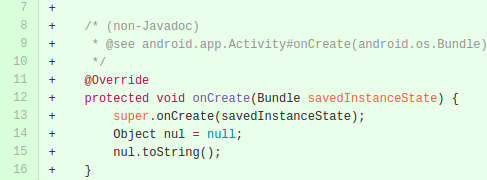
\includegraphics[width=1.0\textwidth]{images/added_example}
    \caption{Newly added method}
    \label{fig:added_method}
\end{figure}

\begin{figure}[!ht]
    \centering
        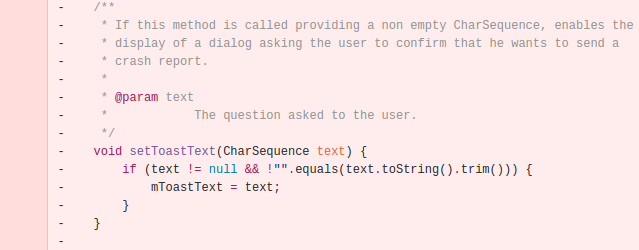
\includegraphics[width=1.0\textwidth]{images/deleted_method}
    \caption{Removed method}
    \label{fig:removed_method}
\end{figure}

\begin{figure}[!ht]
    \centering
        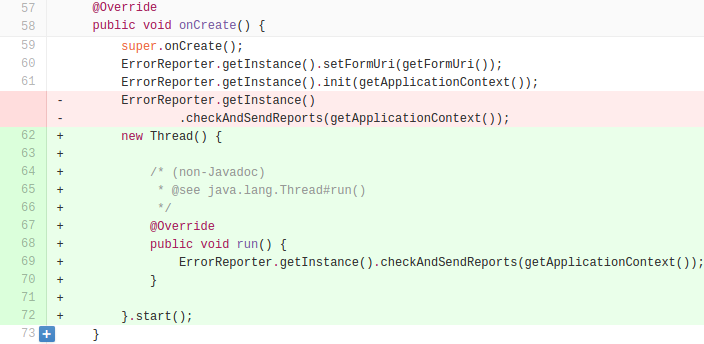
\includegraphics[width=1.0\textwidth]{images/simple_complex}
    \caption{Mixed changed method}
    \label{fig:changed_method}
\end{figure}

\begin{figure}[!ht]
    \centering
        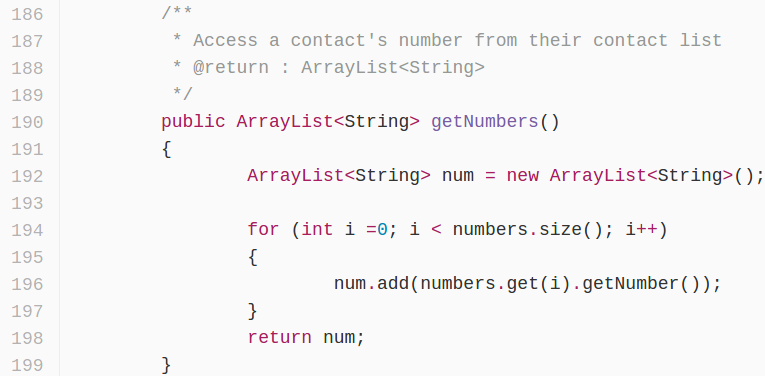
\includegraphics[width=1.0\textwidth]{images/unchanged_example}
    \caption{Unchanged method}
    \label{fig:unchanged_method}
\end{figure}

The process of reconstructing a full file using a patch file requires modifying the original source file. Since the source file used is the product of the patch file the patch must be applied in reverse. Therefore lines with a plus sign, additions, are assumed to be within the file and lines with minus signs, deletions, are assumed to not be present within the file. The lines previous removed from the source file are added back to their original location with a minus sign to preserve the original meaning of the line. The lines that were added to the source file are perpended with a plus sign identify that the line is an addition.

This full source file is then analyzed to extract each method to identify the type of change as well as other method metrics. The type of change that occurred to a method is identified as one of four possible changes. First, a method may be completely new and is thus classified as a new method shown in \autoref{fig:added_method}. The second method closely, related to the first would be an entirely removed method that is classified as a deleted method shown in \autoref{fig:removed_method}. The third classification that is more difficult method to identify is a modified method. Simply a modified method is one that contains at least two of following three change types; added, removed or unchanged lines. An example of a method that contains all three change types is shown in \autoref{fig:changed_method}. In the event that a method consists entirely of additions and deletions then the method is classified as both a new method and deleted method. A deleted and added classification is used over a modified classification because if all lines are deleted and re-added then the method is change far more drastic than a simple modification. The final change type is that of no change, where the method does not contain any changes and is shown in \autoref{fig:unchanged_method}.

For each commit this information is stored to allow for easier access and save time since the analysis of larger datasets can be time intensive. In order to maintain the integrity of the initial dataset this information is stored in a new database. There are several other features available in the data set from the extraction process beyond the ones outlined here in detail. A few of those features include the commit author, the commit message and the method length per commit. This data is stored in the database to help create the prediction model later on.

\section{Visualization}

\subsection{Line Change}
\label{subsec:line_change}

After collection and analysis of the data is complete the key features are extracted. Visualizations were used in order to to better understand resulting data. The first visualization simply showed the changes recorded on a per line basis. These changes were divided into several closely related subcategories of additions, deletions and modifications. Additions identify changes that are new and do not have a corresponding set of deleted code. Similarly deletions refers to changes that remove lines of code without a corresponding set of additions. Finally modifications are a set of changes which contain a set of additions and deletions that are related.

% \lstloadlanguages{Ruby}

% \definecolor{codered}{rgb}{1.0,0.0,0.5}
% \definecolor{codegray}{rgb}{0.5,0.5,0.5}
% \lstset{%
%     label=listing:levenshtein_distance,
%     float=h,
%     caption=levenshtein.rb,
%     firstnumber=1,
%     language=Ruby,
%     basicstyle=\ttfamily,
%     keywordstyle=\color{codered},
%     stringstyle=\color{yellow},
%     numberstyle=\color{codegray},
%     commentstyle=\color{codegray}}

% \lstinputlisting[language=Ruby]{listings/levenshtein.rb}


The relationship between two sets of additions and deletions is determined through the \gls{ld} formula. The \gls{ld} distance calculation will determine the edit distance between two strings. Where edit distance is defined as the number of characters difference between two different strings. For example, the \gls{ld} for \textit{happy} and \textit{mapper} would be 3, since h would be changed to m, y to e and r would be added at the end. While this provides a good initial method for comparison between two string values the value need be normalized to allow for more general use. To calculate \gls{nld} the \gls{ld} would be divided by the larger of the two strings sizes shown in \autoref{eq:normalized_ld}.

% TODO note that a_i is an addition line and that d_j is a deletion line
% TODO clarify change block with picture

\begin{equation}
\label{eq:normalized_ld}
NLD(a_i, d_j) = \frac{LD(a_i, d_j)}{\max(|a_i|,|d_j|)}
\end{equation}

% TODO show distance calculation and paper cite this.
Line modifications are assumed to only take place in a series of line changes that involved both additions and deletions shown in \autoref{fig:changed_method}. In this example, 3 line modifications take place each containing 1 addition and 1 deletion. A line modification can also have an $|a|$ to $|d|$ relationship. That is to say more generally, $|a|$ lines of addition may relate to $|d|$ lines of deletion where both $|a|, |d| > 0$. In order to determine whether two lines are closely related enough a threshold $\Delta_m$ is defined. As outlined in \autoref{eq:similarity_threshold}, when the \gls{nld} is below the threshold $\Delta_m$ then the two lines are related.

\begin{equation}
\label{eq:similarity_threshold}
m(a_i, d_j) = NLD(a_i, d_j) < \Delta_m
\end{equation}

Normalizing the \gls{ld} calculation accounts for the differences in line sizes when being compared. With shorter lines, the change of a variable name could change a large portion. Therefore with smaller lines likely modifications result in a dramatically higher distance between lines. Likewise, longer lines can contain more text modifications and still result in a low score because of the length of the line. This resulted in the creation of the a threshold $\alpha$ to separate small and large line changes. The \autoref{eq:similarity_threshold} is updated accordingly shown in \autoref{eq:complete_similarity_threshold}.

\begin{equation}
\label{eq:complete_similarity_threshold}
m(a_i, d_j) = \left\{\begin{matrix}
NLD(a_i, d_j) < \Delta_s & \text{if } \max(|a_i|, |d_j|) < \alpha \\ 
NLD(a_i, d_j) < \Delta_l & \text{otherwise}
\end{matrix}\right.
\end{equation}

Only lines that are part of the same block of additions and deletions are selected for the similarity check to determine whether they can be classified as a modification. As noted before line modifications will consist of one to many addition lines mapped to one to many lines of deletion. Therefore a modification is more easily referred to as a modification set. For addition lines that do not meet the threshold of similarity with all deletion line in the change block are classified as additions. Similarly, deletion lines that fail to meet the similarity threshold for all addition lines will be classified as deletions. Therefore a block of changes will contain a set of additions, deletions and modifications any of which may be empty.

% comments.
While creating the parsing method both code and comments were considered separate entities. However each was analyzed with the same method. Therefore for the visualization below the changes are separated into source code and comments. The comments were never used towards the prediction method presented later on in \autoref{chap:prediction} and will therefore not be covered as deeply. The comments however are available for use and could be used to extend the approach.


% Discuss the slight controls that each one allows and the special one just for this view. TODO place this better.
Each of the following visualizations presented have a interactive component which is not available. Their capabilities are summarized to provide context to their use. The line change data is visualized in \autoref{fig:line_visual_acra}. The number of changes lines of source code added, deleted and modifications are all shown aggregated per month. A per commit view is available but is very cluttered because of the excess of data with in a project. The bottom half of the visualization shows the sum of changes up till the given point. Tags for the project are shown at the bottom of the graph to provide some context of the release cycle. Tags often mark points of significance within the project and therefore can be thought as road signs. The visualization also provides some options to refine or generalize the view. For all of the views the user is allowed to select the project, package path, and the committers as desired. Specifically for the line level graph a further option is provided to condense the data based on a monthly, weekly and commit summary. The commit message and a link to the commit on GitHub is provided when viewing either the commit view, method level or statement level. This information allows for a direct link to the project and can be a handy tool for referring back to the software repository.

Each view is also supplemented with a summary of key stats for the project. In \autoref{fig:project_summary_stats} the project stats are outlined for \textit{acra}. The ratio of comments to code for the history of the project is shown in a pie chart. Several table entries outline several top performers metrics are outlined with the top five for each category. The first set outlines top contributers for source code, which is broken down into the categories: coder, modifier and deleter. Coder, modifier and deleter all map to the top committer to provide additions, modifications and deletions respectively. The number of line added is also outlined as well next to the committer's name in square brackets. The second set of lists outlines the top commenters for additions, modification and deletions. Finally, the top committers and contributors are listed, where the committer is sum of commits contributed to the project, and contributer is the sum of total code and comments contributed.

% \begin{figure}[!ht]
%     \centering
%         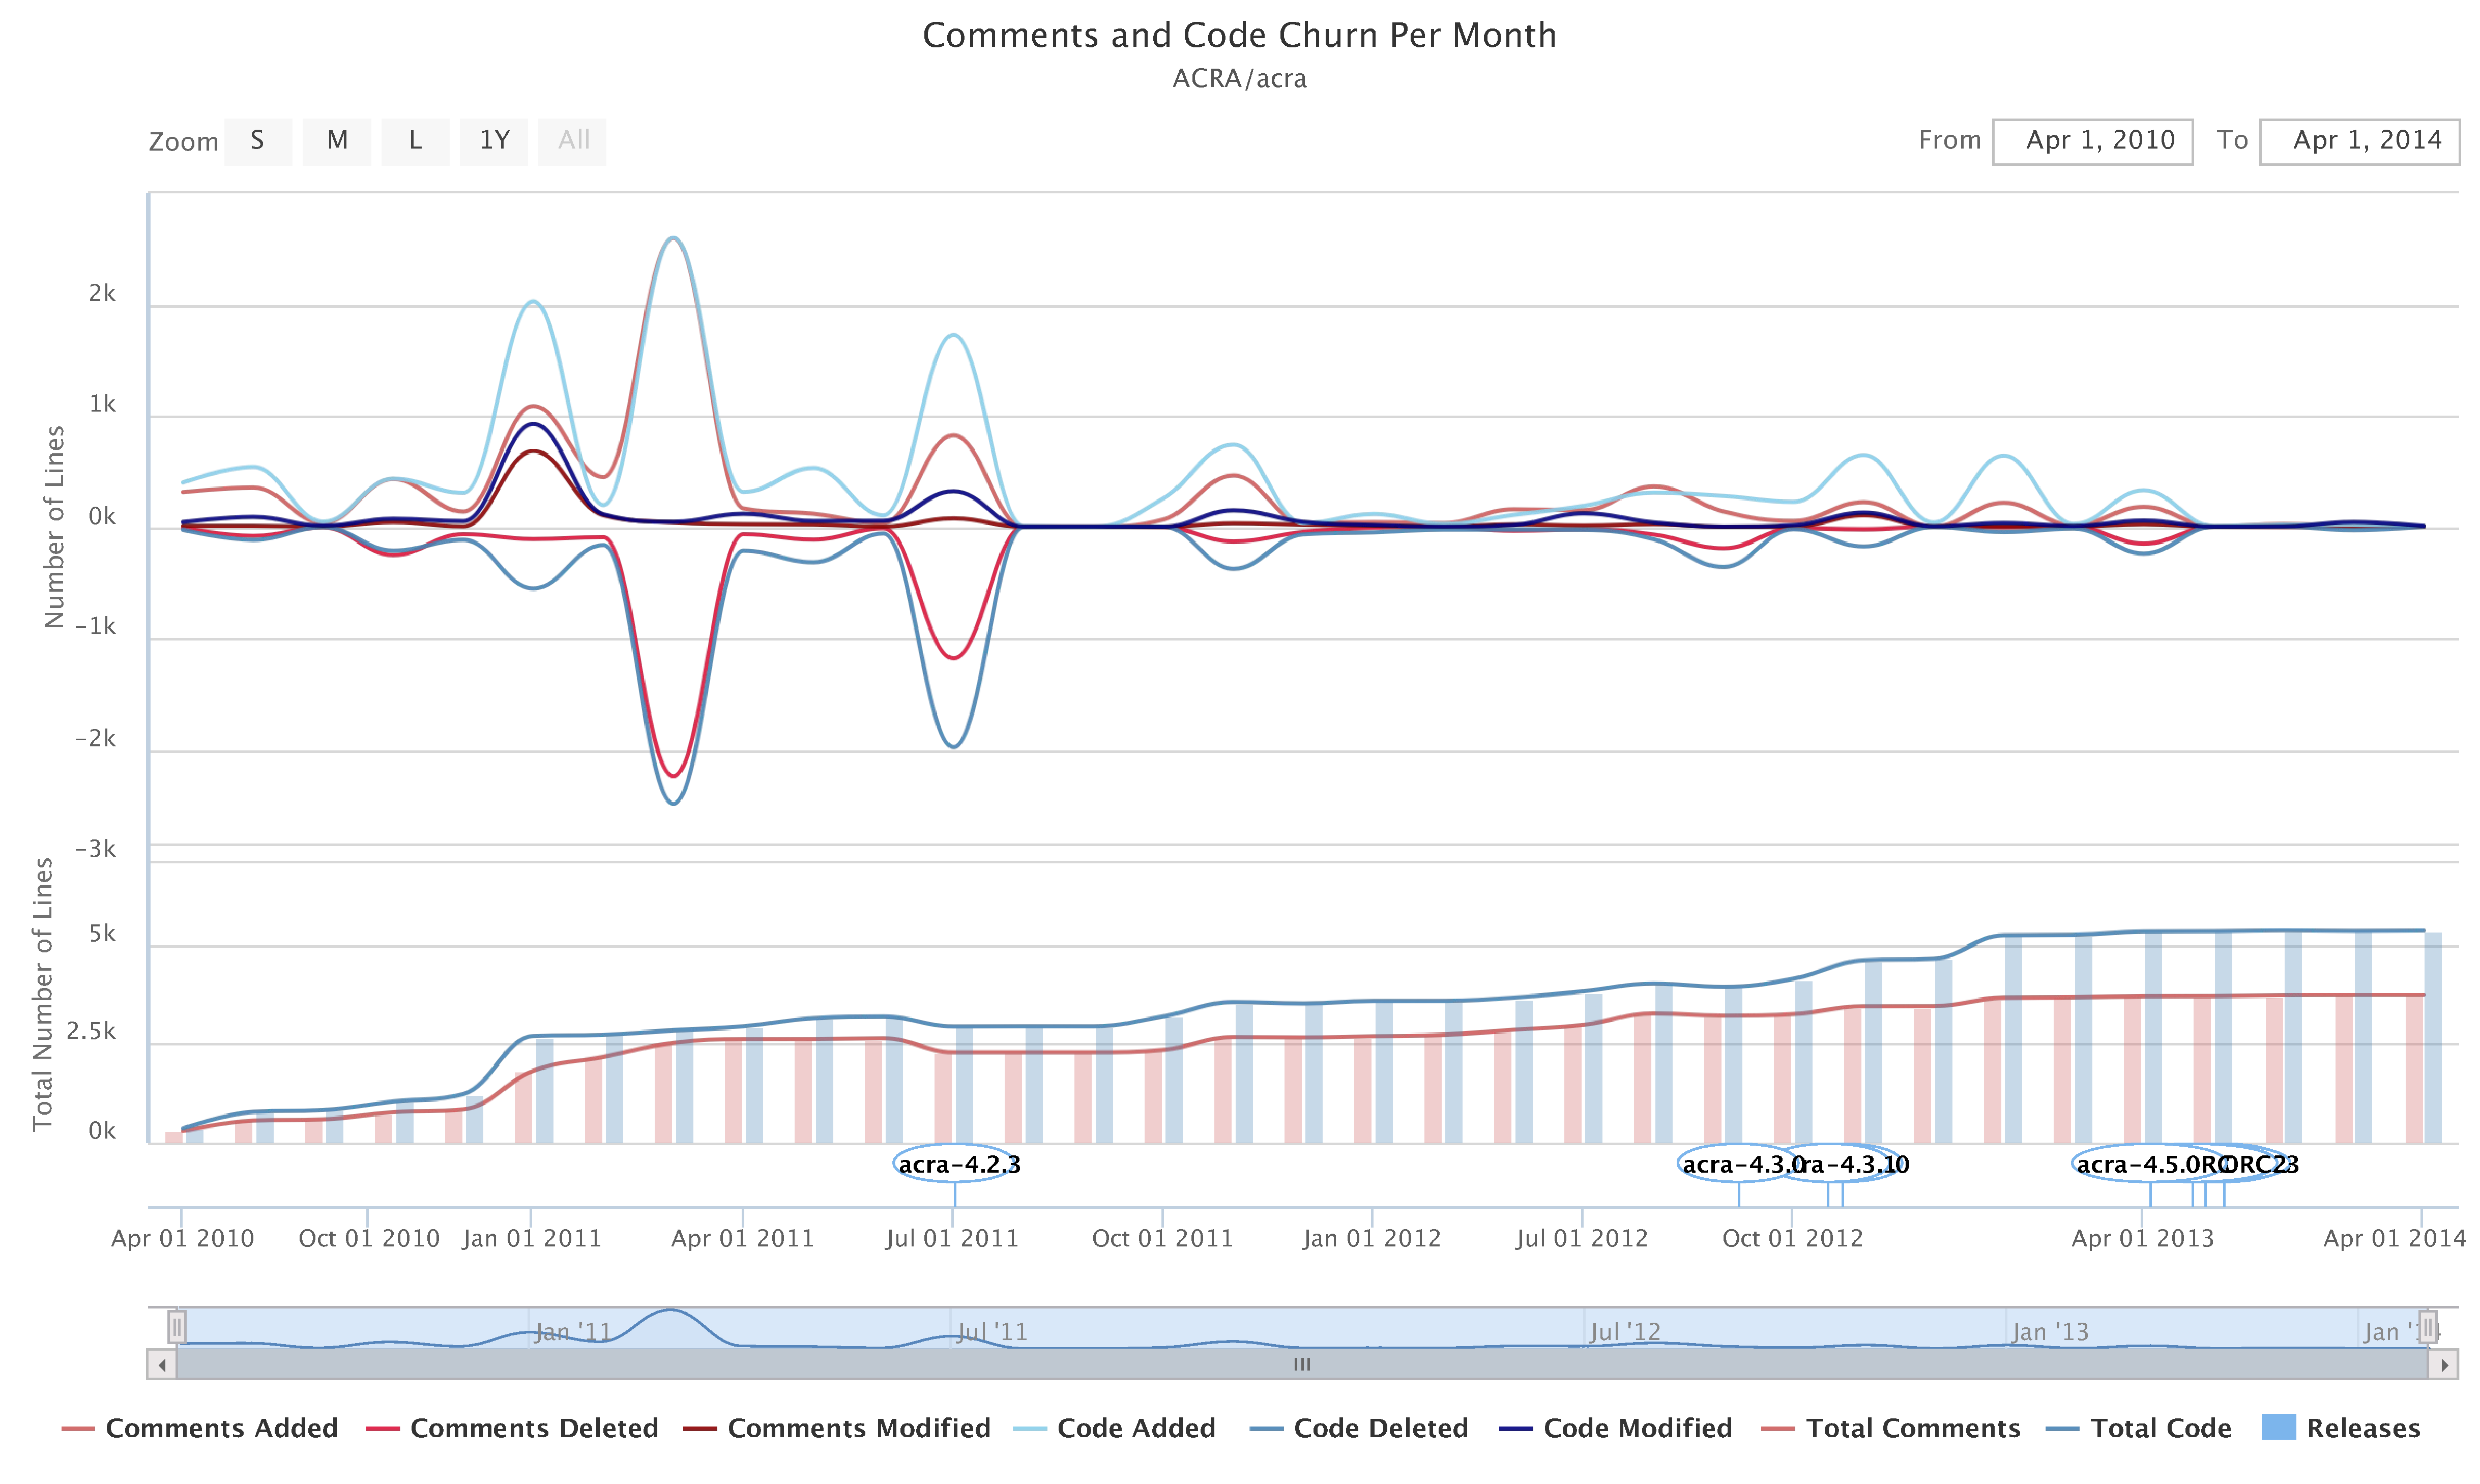
\includegraphics[width=1.0\textwidth]{images/lines_visual_acra}
%     \caption{Line Change Visualization for acra}
%     \label{fig:line_visual_acra}
% \end{figure}


\begin{landscape}
 \thispagestyle{empty}
 \begin{figure}
  \centering
        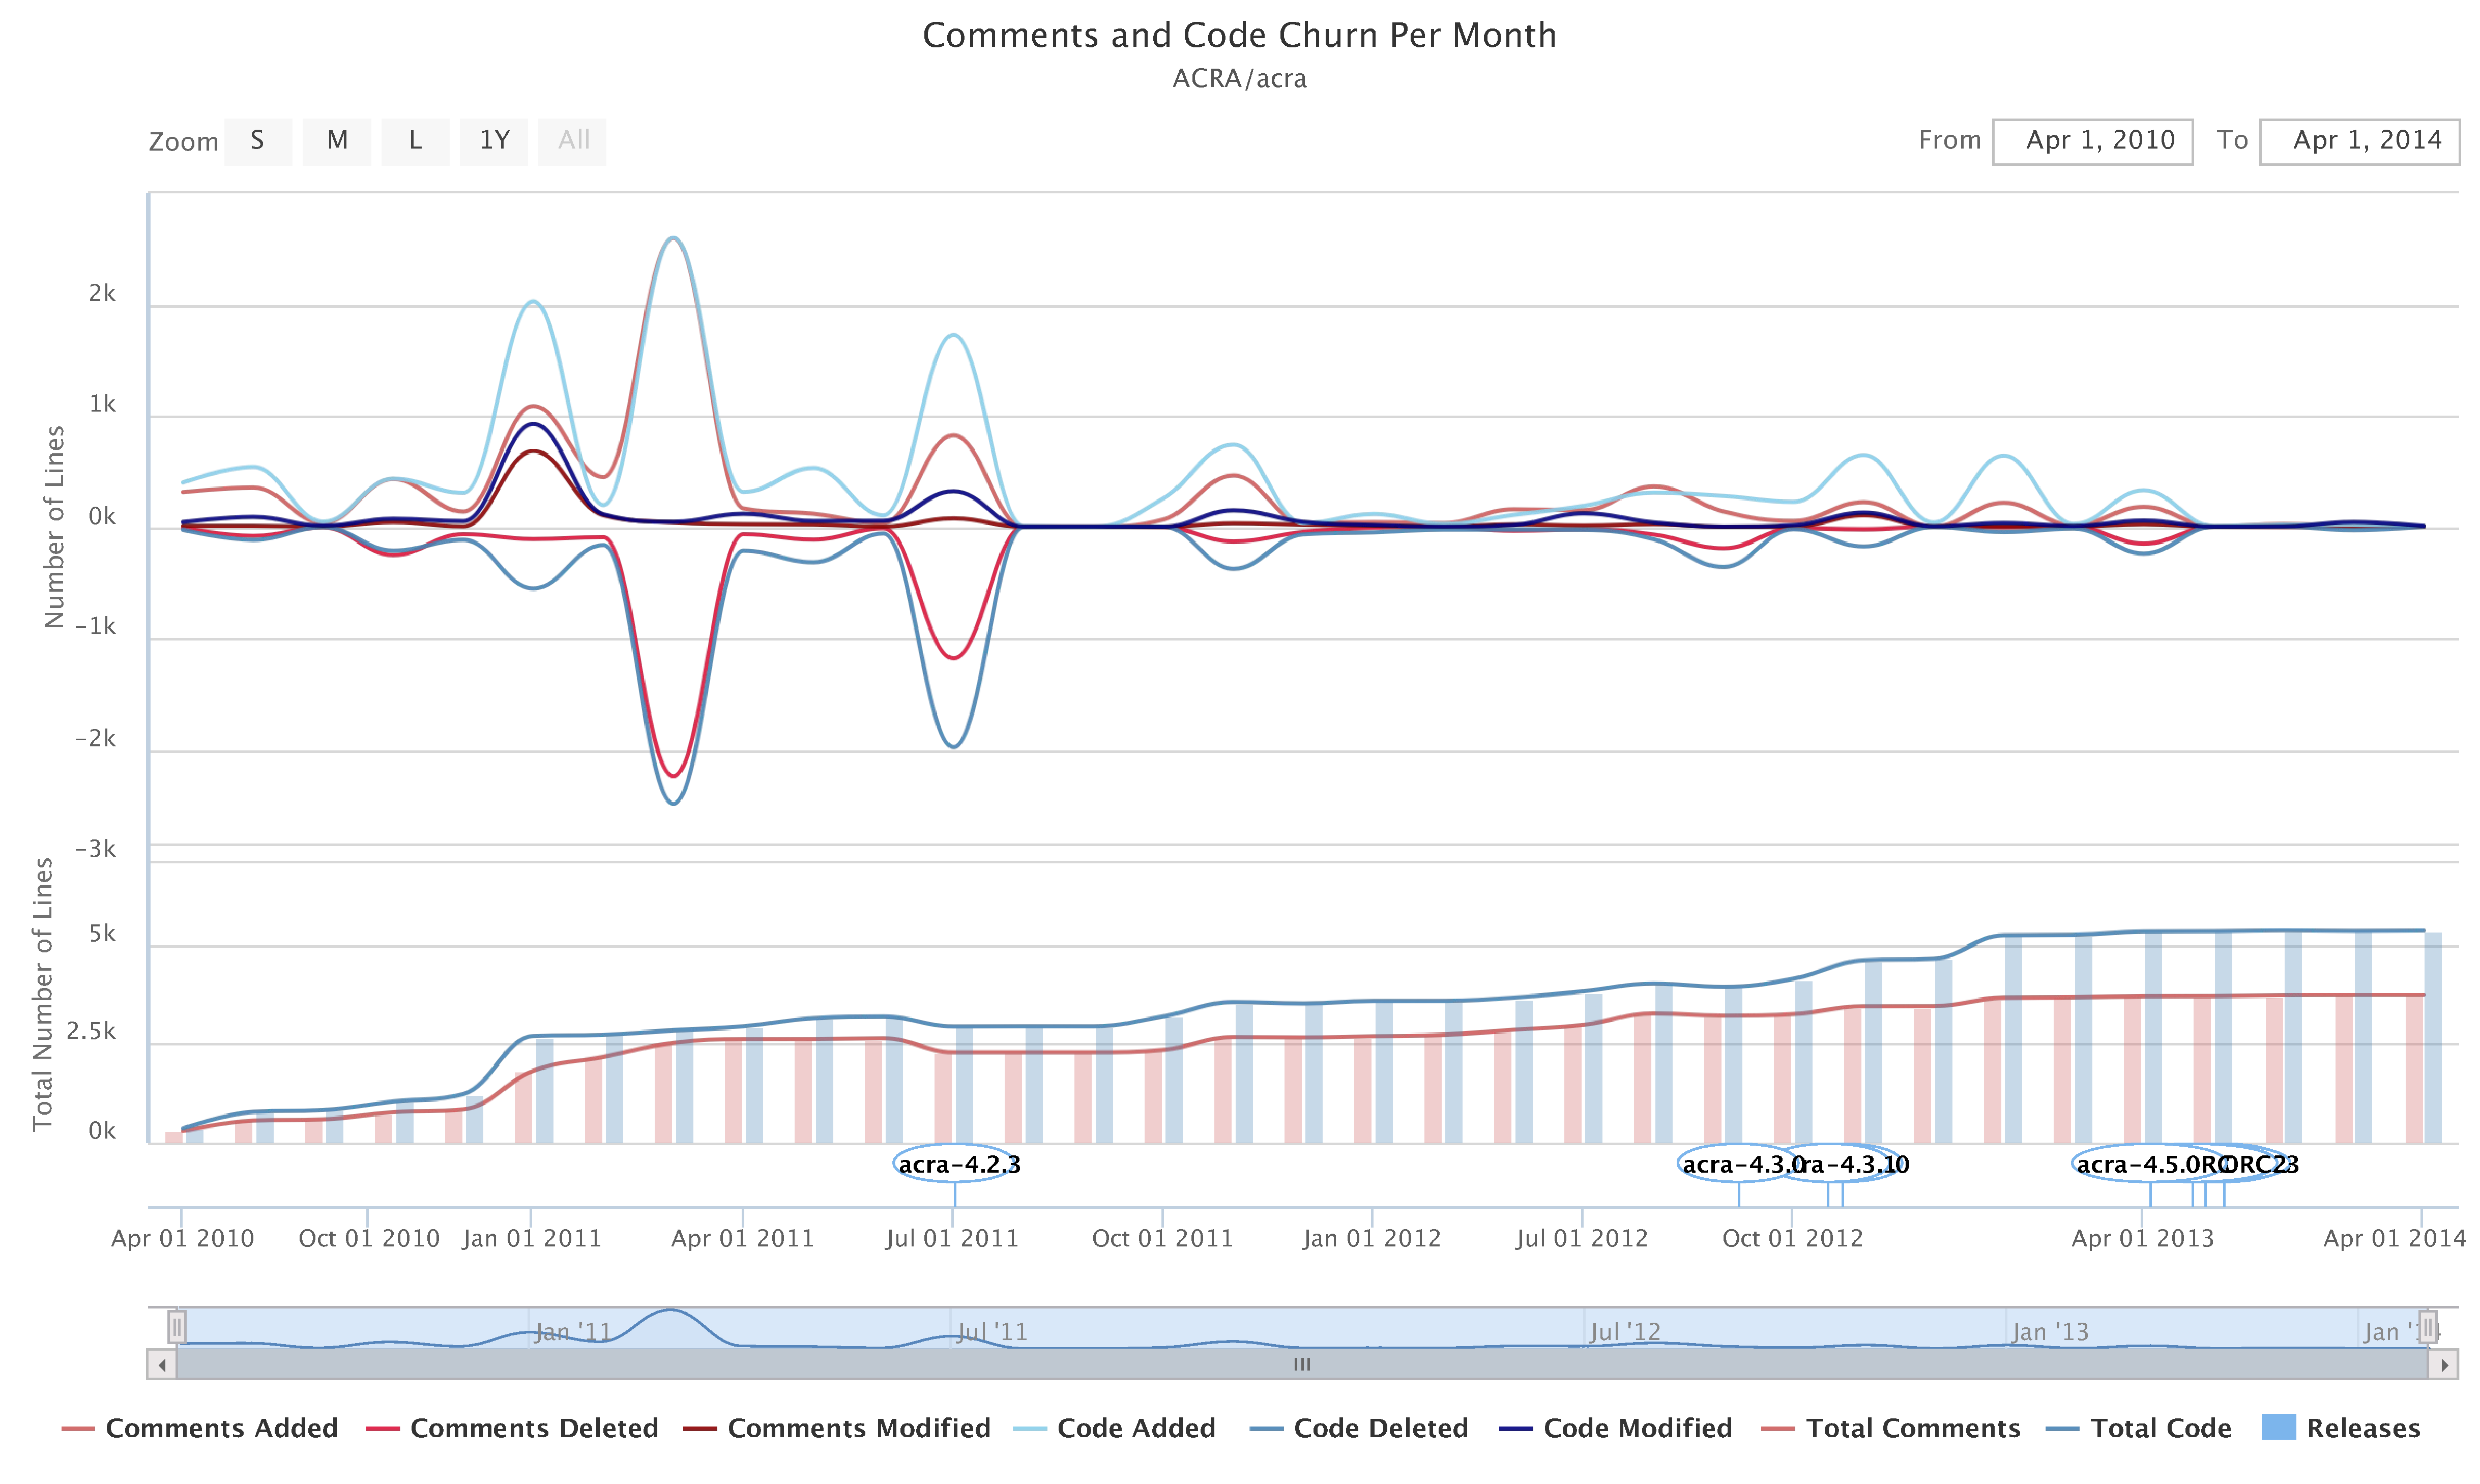
\includegraphics[width=1.5\textwidth]{images/lines_visual_acra}
    \caption{Line Change Visualization for acra}
    \label{fig:line_visual_acra}
 \end{figure}
\end{landscape}
\pagestyle{plain}

% TODO put this in the right location
% TODO talk about this.
\begin{landscape}
\thispagestyle{empty}
 \begin{figure}
  \centering
        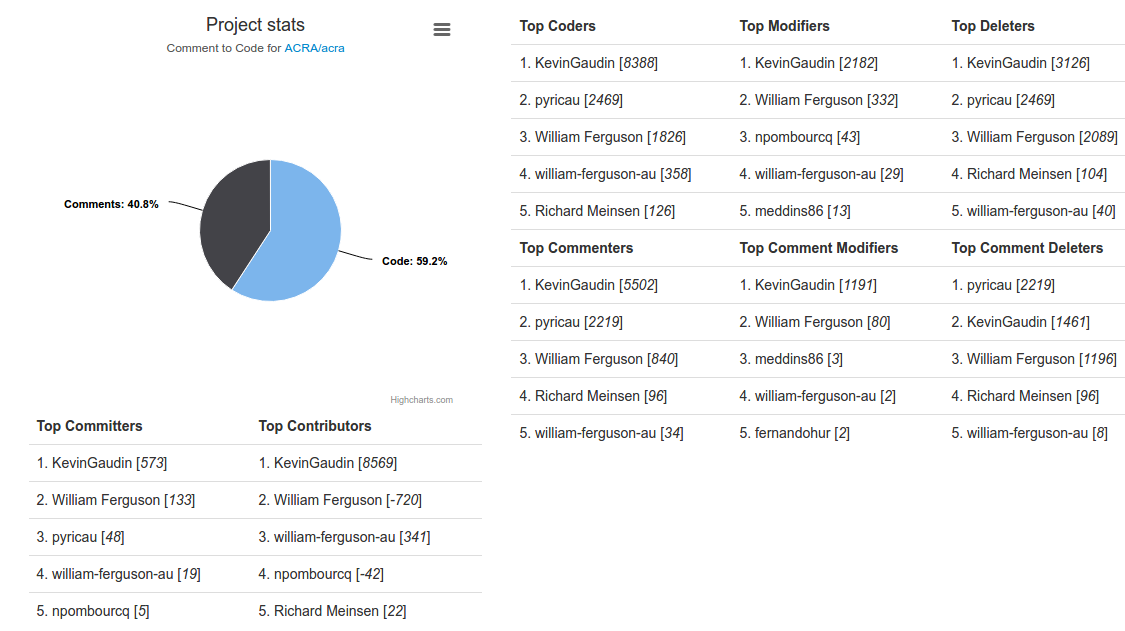
\includegraphics[width=1.5\textwidth]{images/table_visual}
    \caption{Project Summary Statistics for acra}
    \label{fig:project_summary_stats}
 \end{figure}
\end{landscape}
\pagestyle{plain}

\subsection{Method Change}

The visualization of line changes was very noisy and proved difficult to use. Instead of viewing every line of change separately, the changes are grouped together based on the method from which they originate from. Similar classifications are used for method changes however their definitions vary slightly and are outlined in more detail in \autoref{sec:parsing}. There are three types of method level changes that can occur. Firstly, a method is classified as newly added when that the method had not existed in the previous version, consisting only of additions. Secondly, a deleted method implying that the method is completely removed from the current version, consisting only of deletions. Thirdly, a method is classified as modified if it contains two or more types of changes, either additions, deletions or no change.

The method level change visualization, shown in \autoref{fig:method_visual_acra}, presents the amount of method changes that occur in the project development over time for acra. The low level changes details are ignored in this view, instead the focus is placed on that of the three types of changes. The visualization for the method level uses a bar graph since it provided a more clear picture of the relationship between commits. Compared to the first visualization which implied that a relationship between different commits of the same type of changes. The contrast in magnitude between each type of change and each commit is also more clear and defines the visualization. The amount of change occurring over time is clearly visible and the amount of data available is not as overwhelming as the line change visualization.

% \begin{sidewaysfigure}[ht]
%     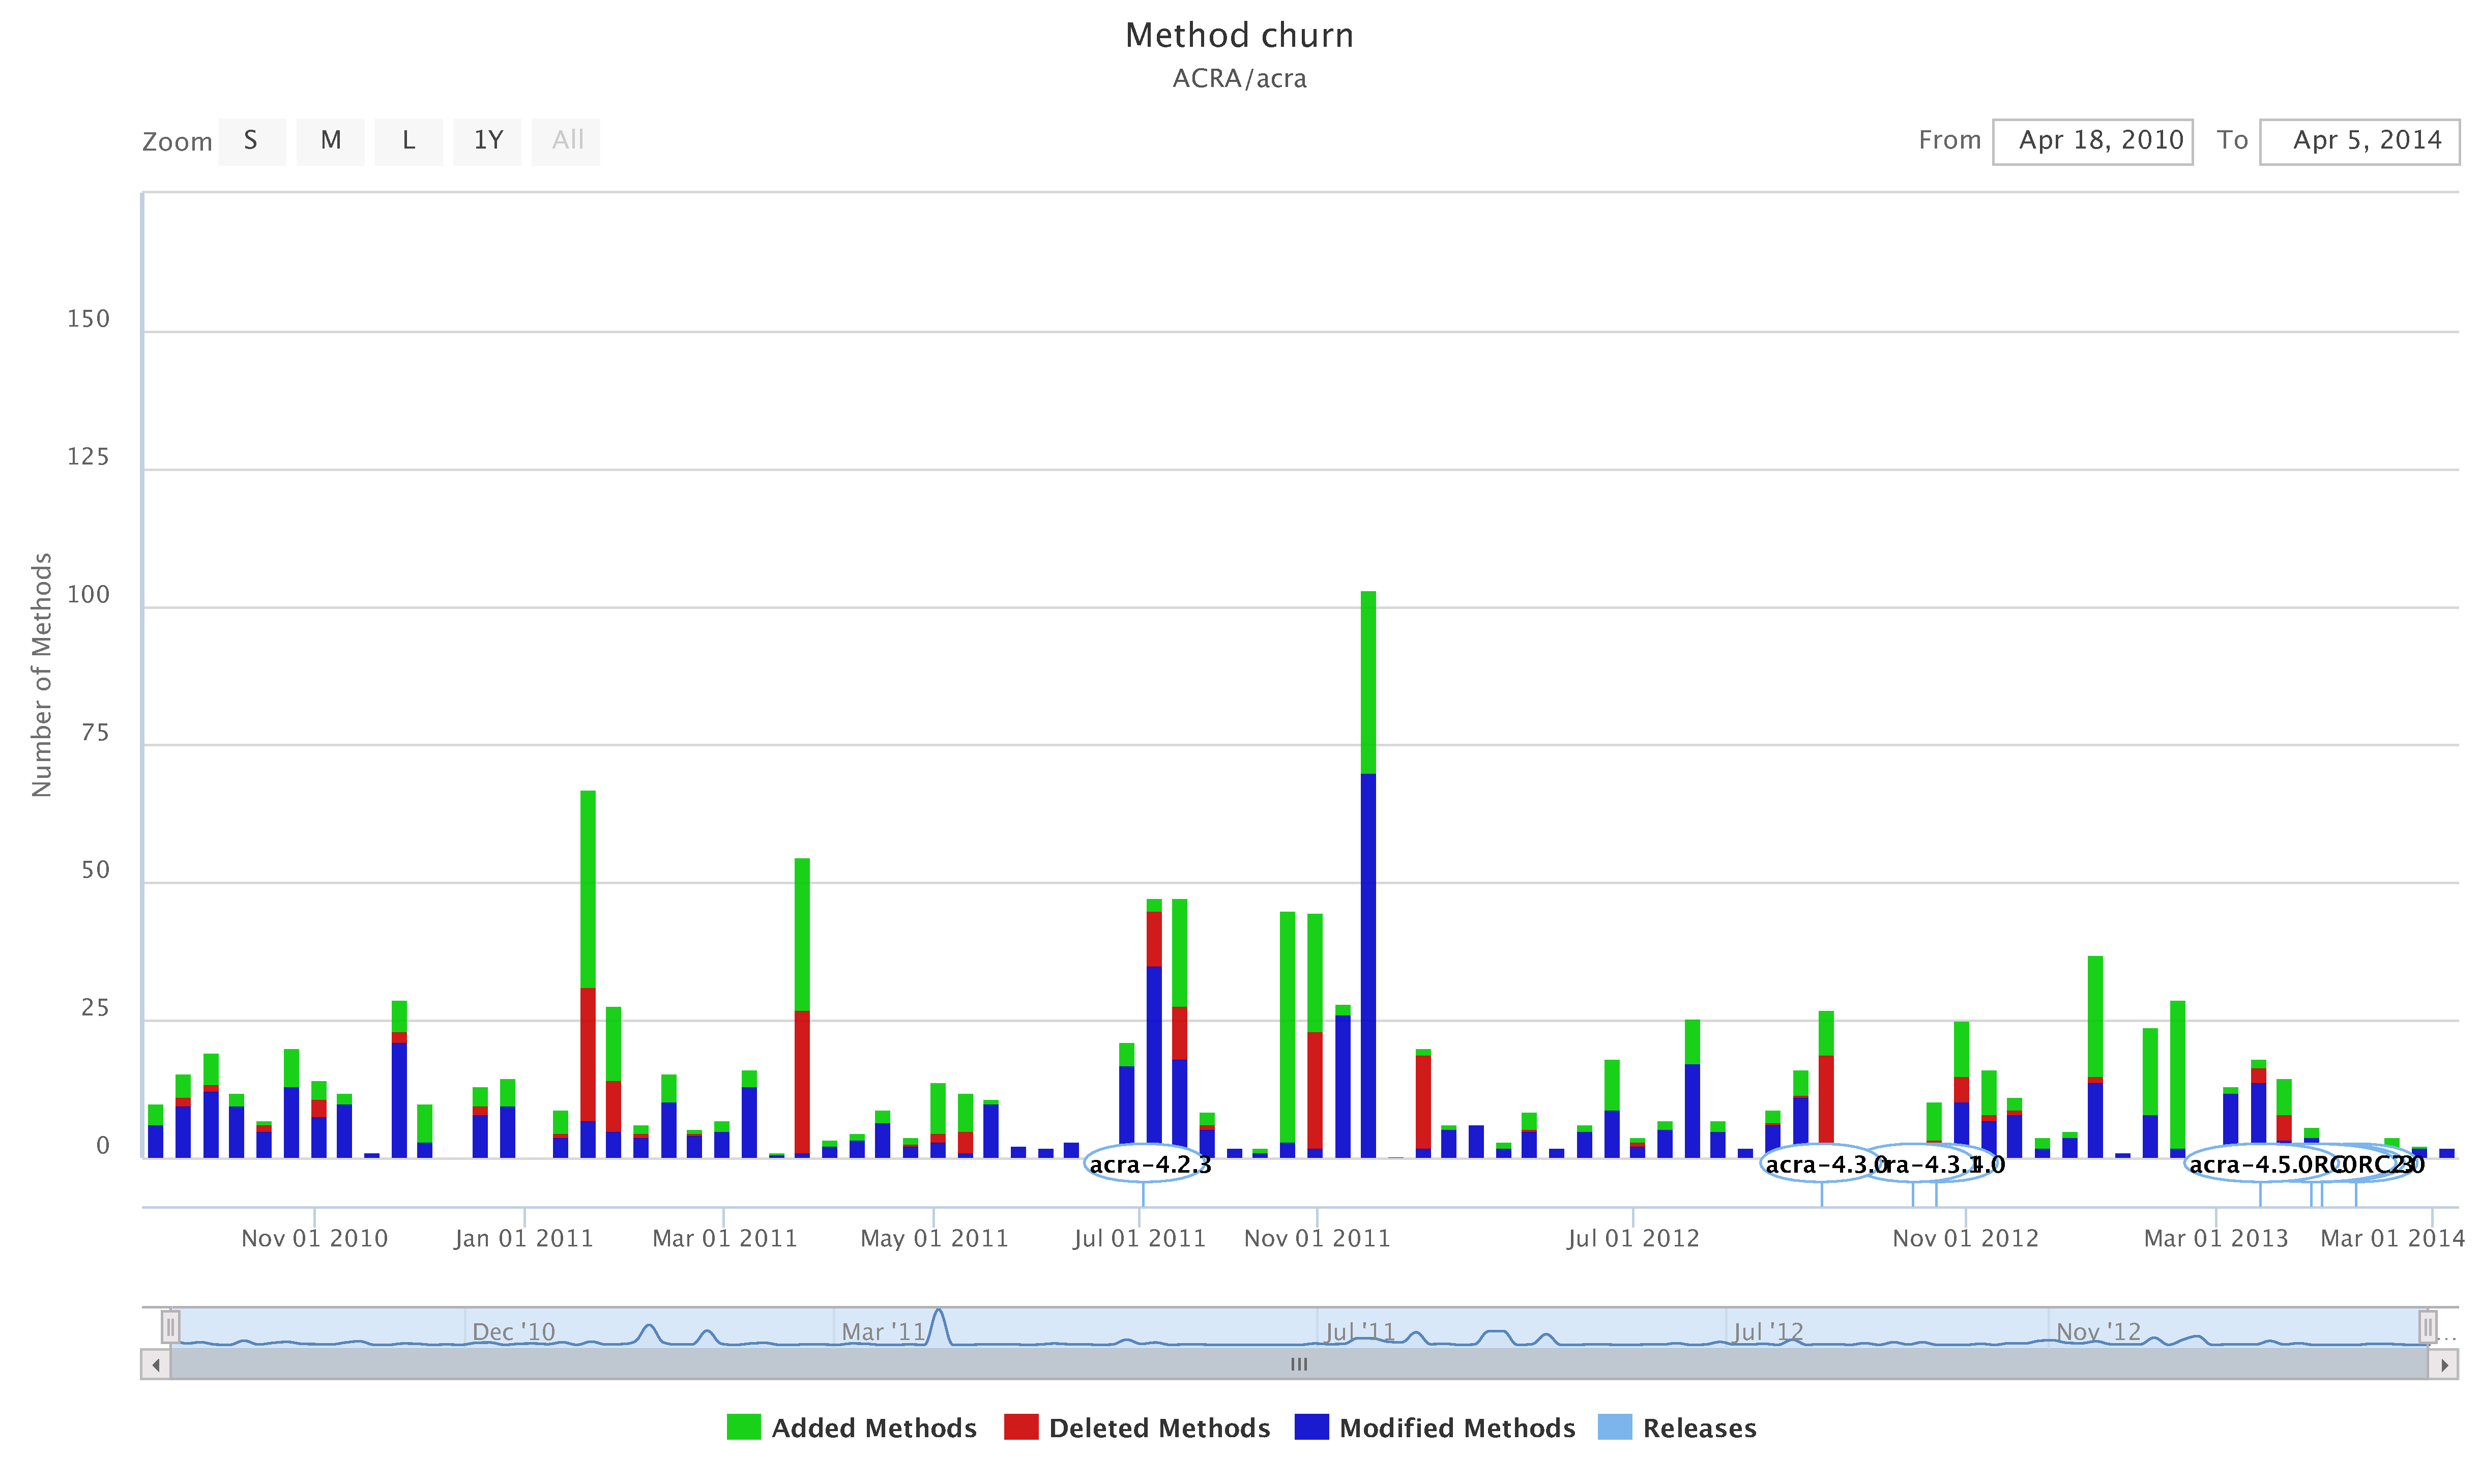
\includegraphics[width=1.0\textwidth]{images/method_visual_acra}
%     \caption{Method Change Visualization for acra}
%     \label{fig:method_visual_acra}
% \end{sidewaysfigure}

\begin{landscape}
\thispagestyle{empty}
 \begin{figure}
  \centering
    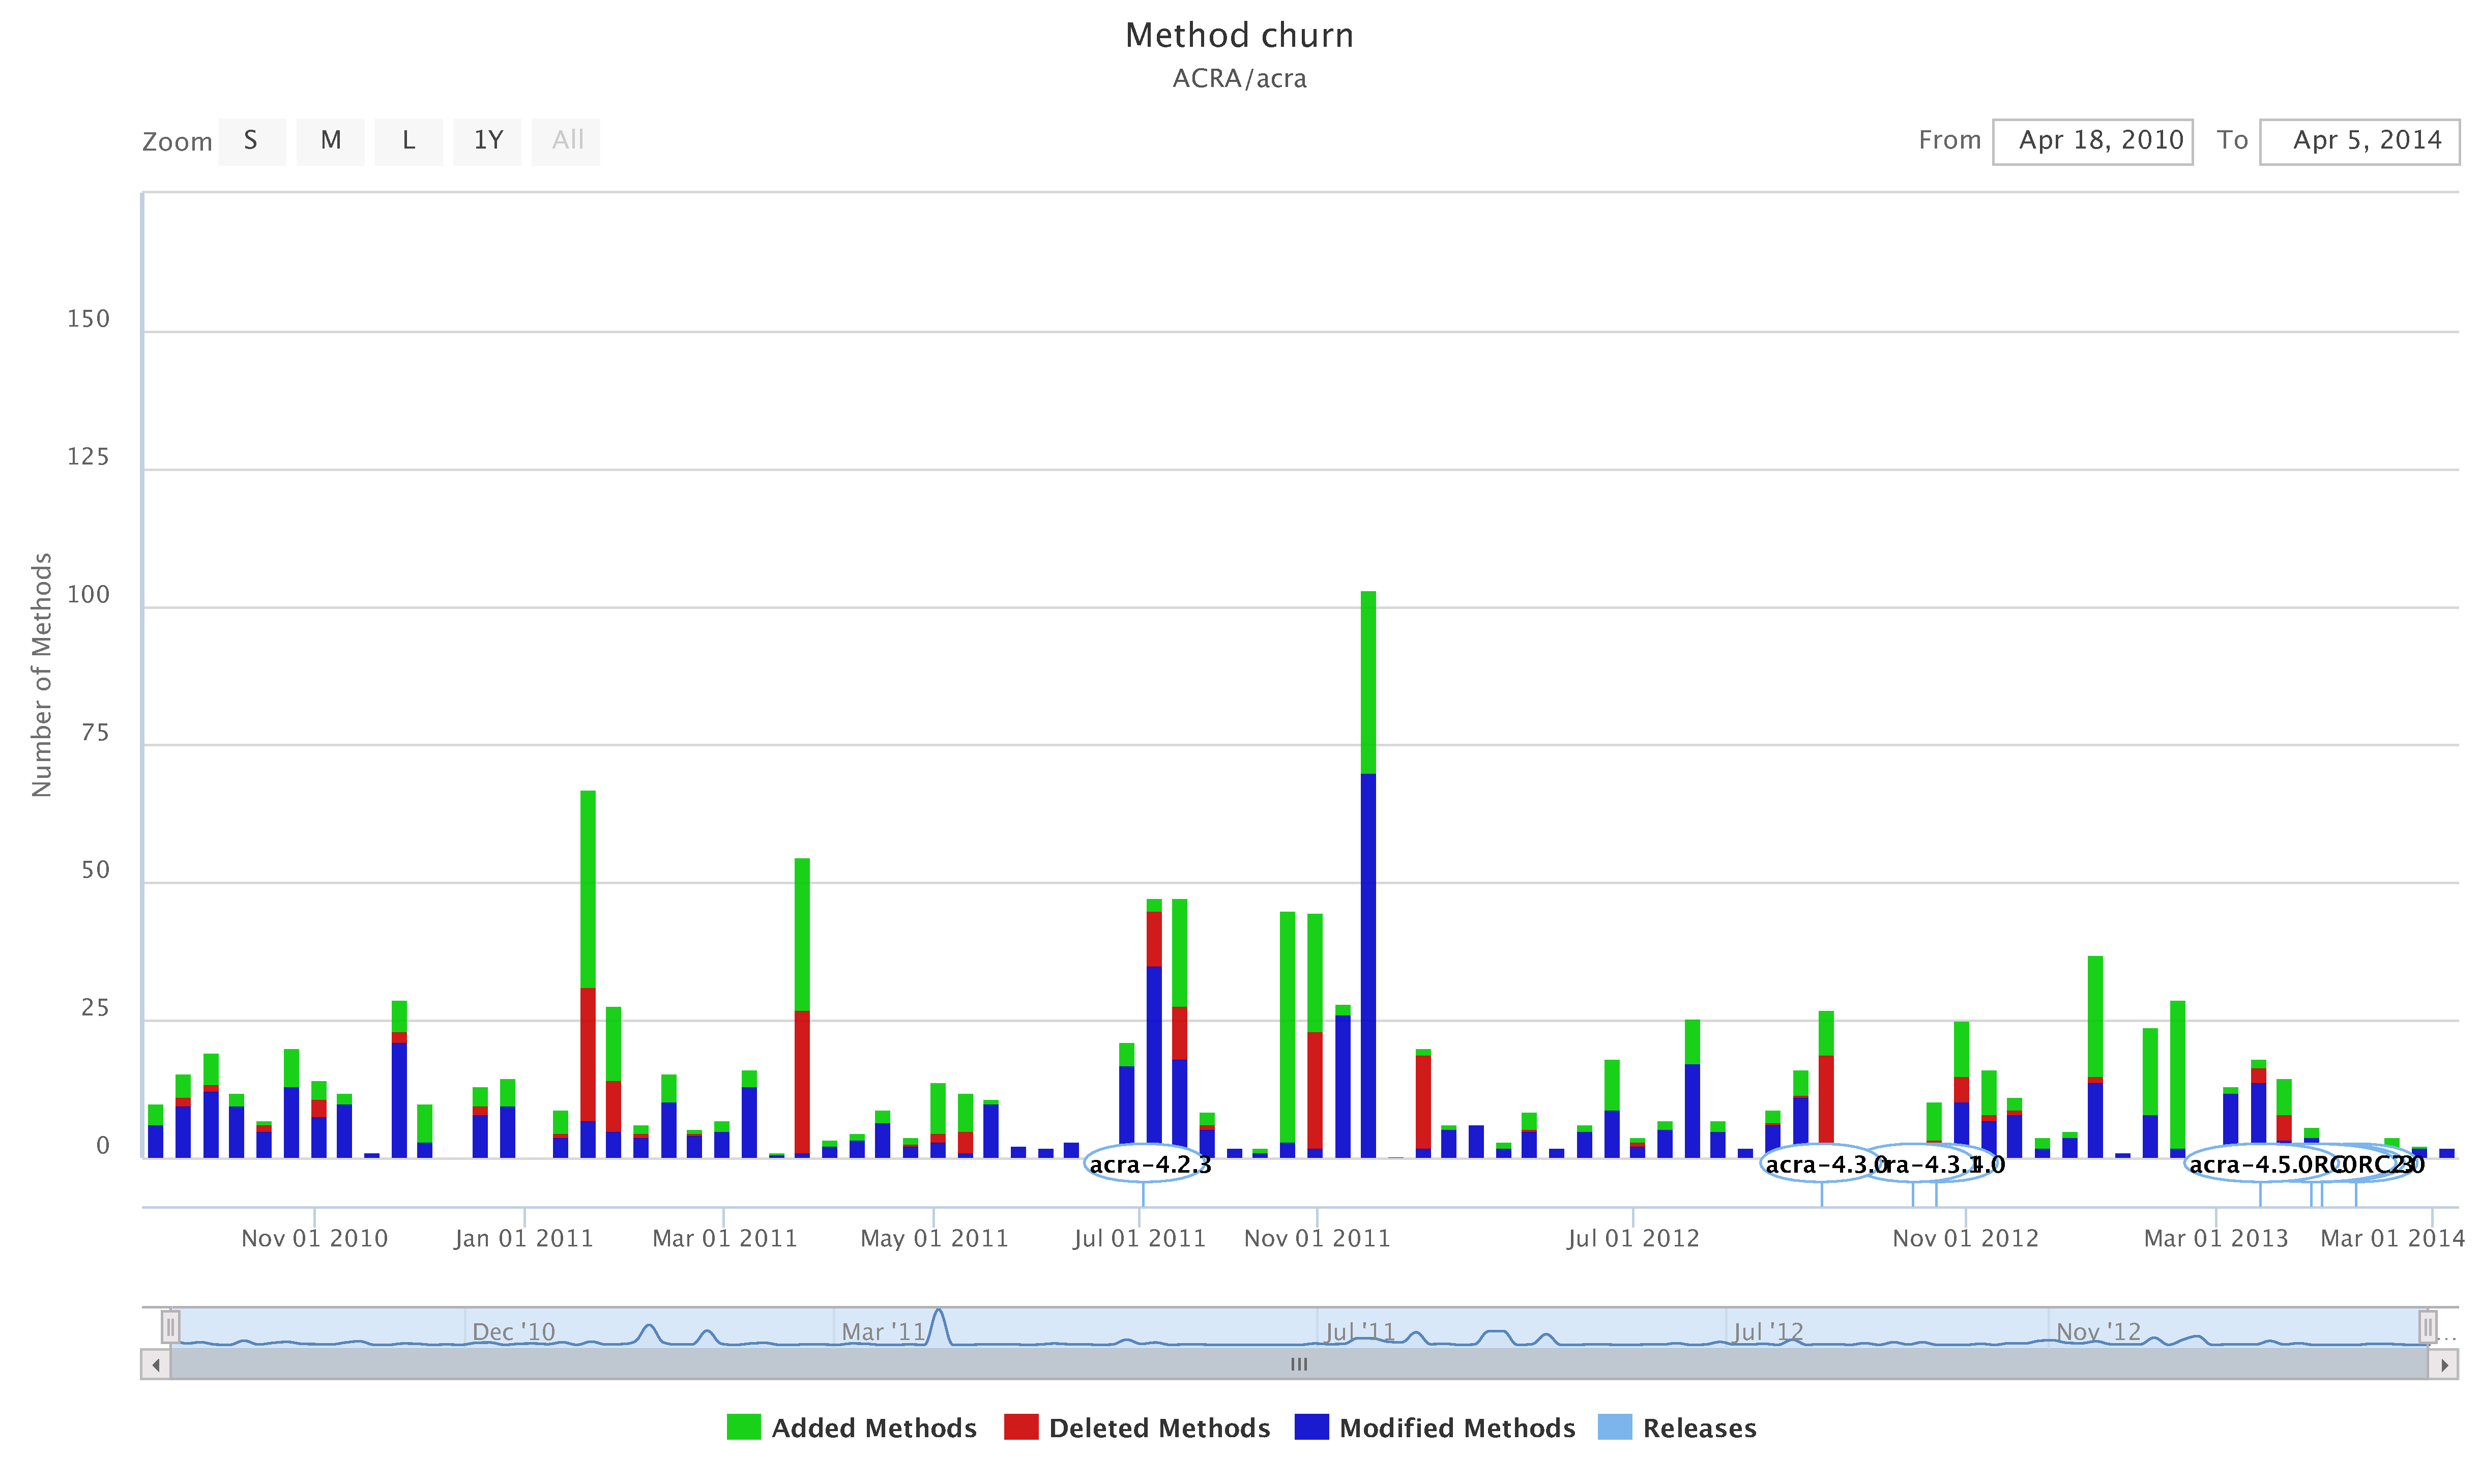
\includegraphics[width=1.5\textwidth]{images/method_visual_acra}
    \caption{Method Change Visualization for acra}
    \label{fig:method_visual_acra}
 \end{figure}
\end{landscape}
\thispagestyle{plain}

% \begin{figure}[!ht]
%     \centering
%     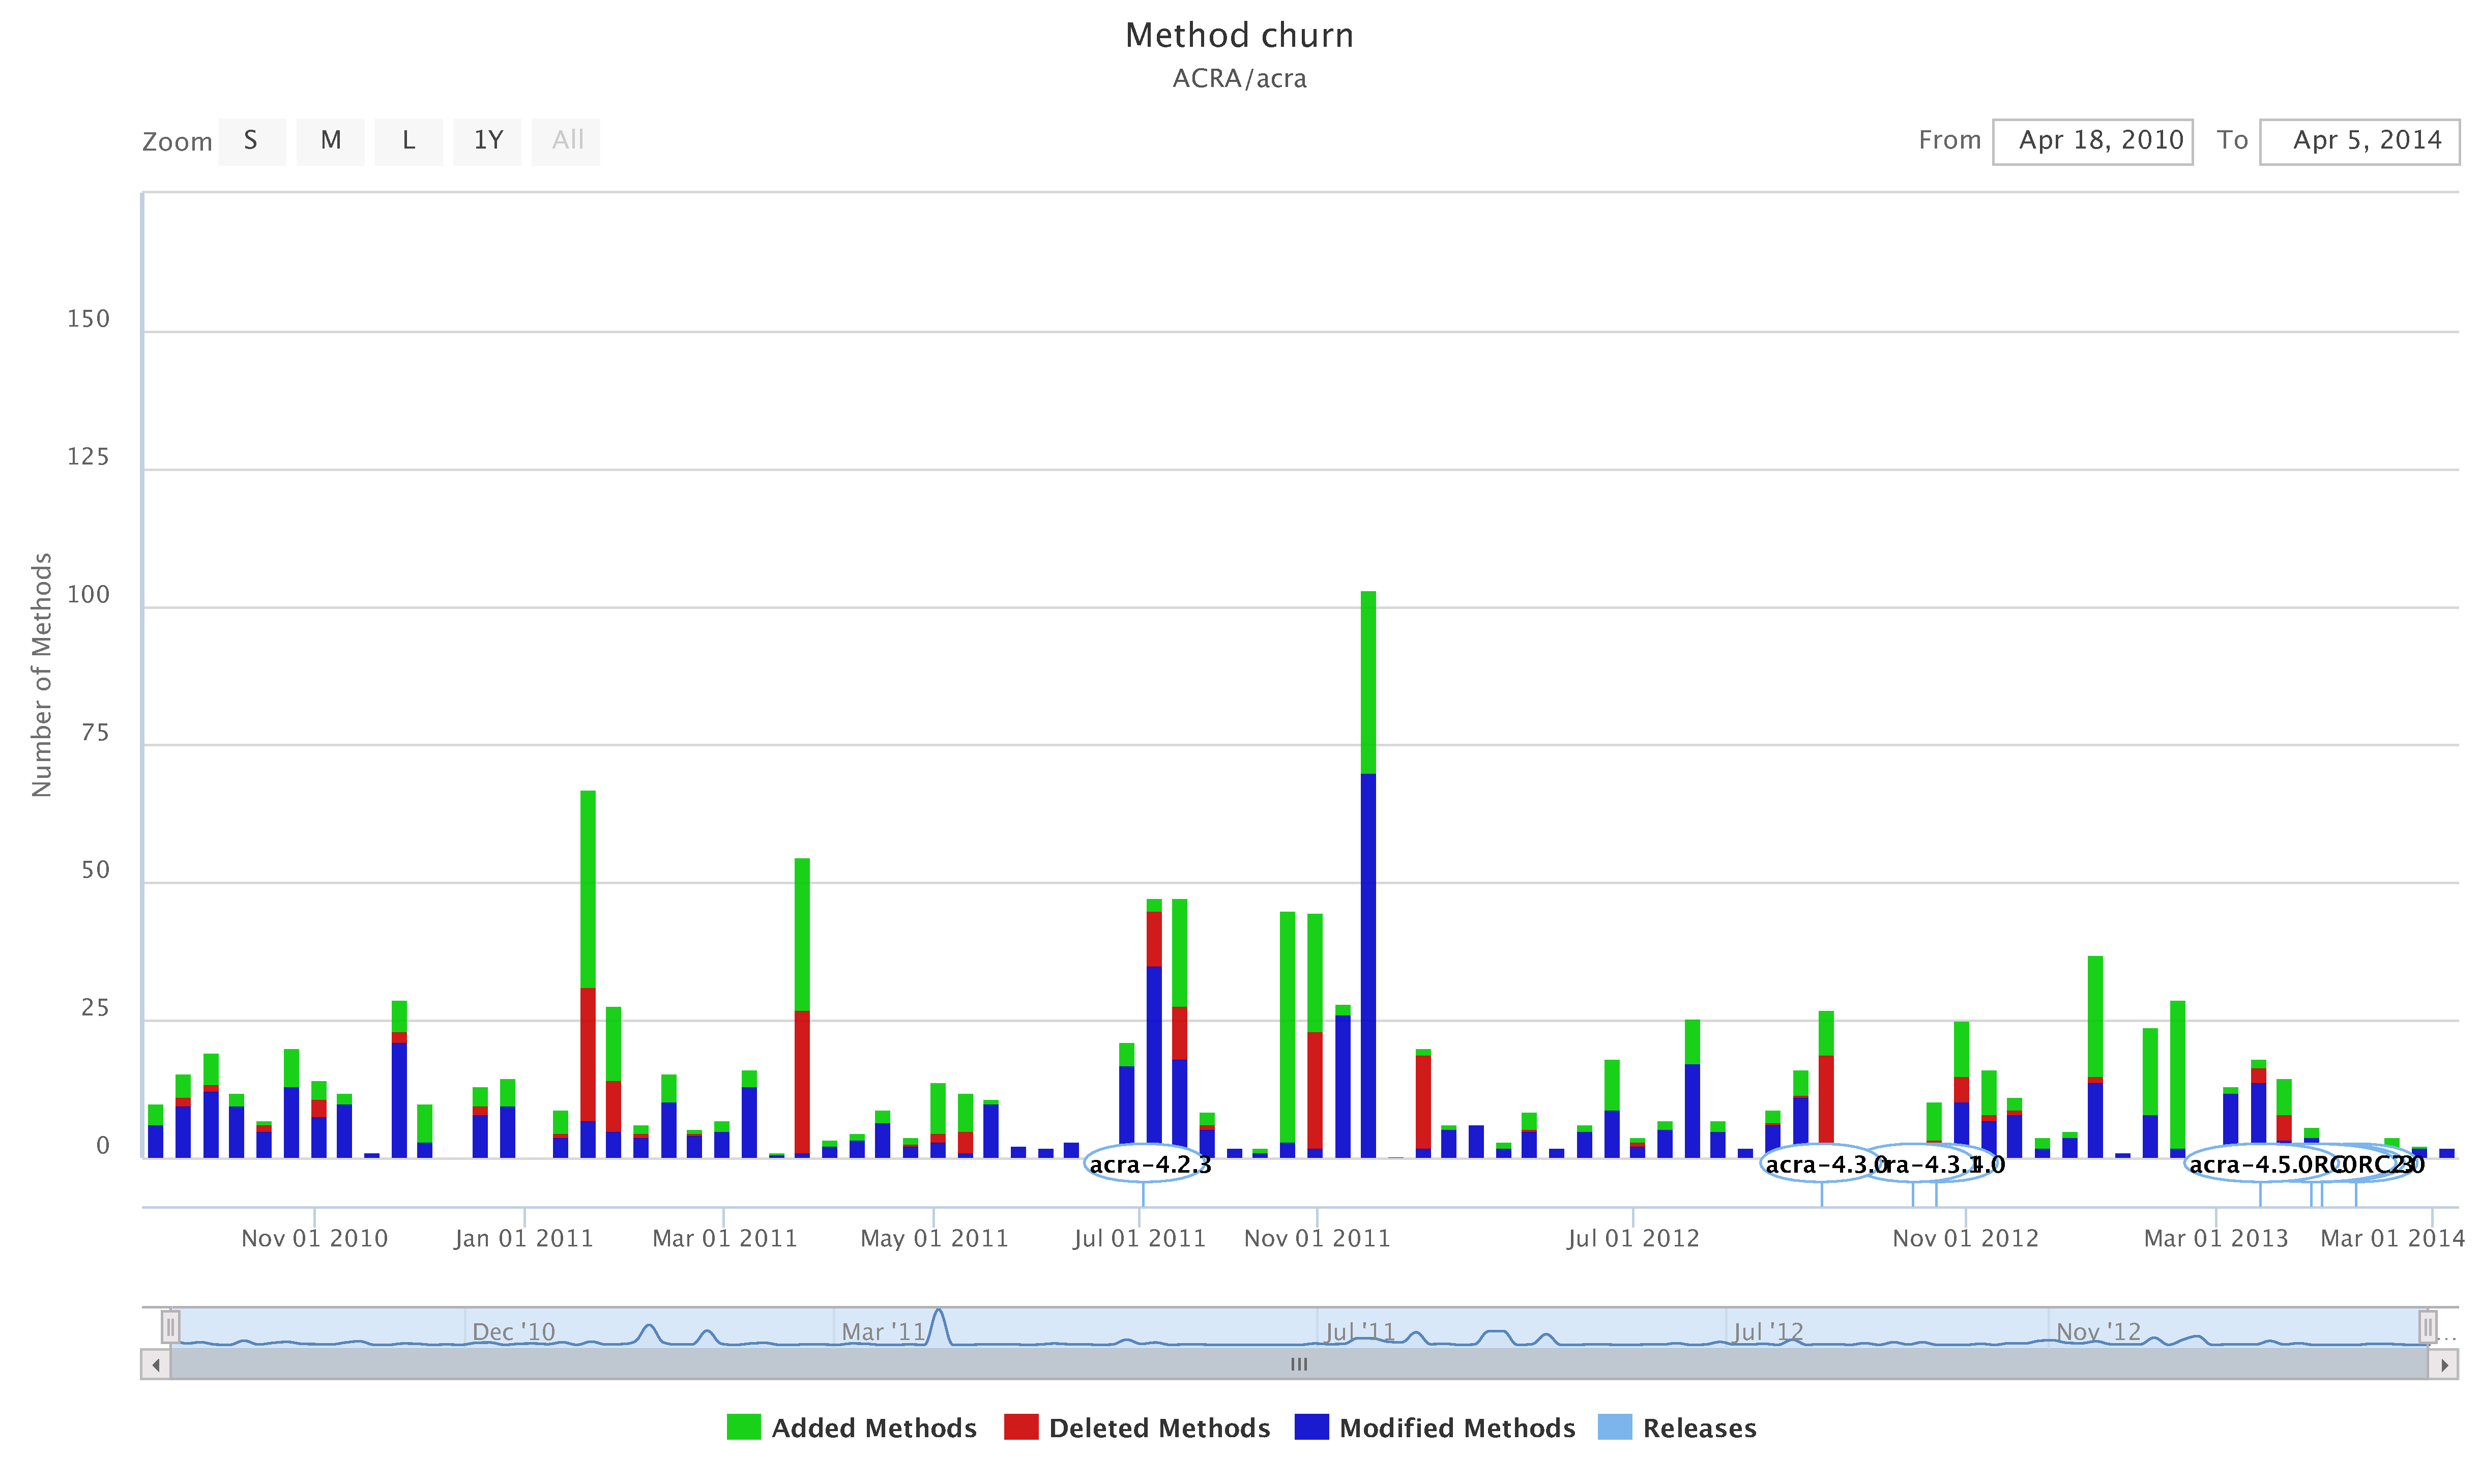
\includegraphics[width=1.0\textwidth]{images/method_visual_acra}
%     \caption{Method Change Visualization for acra}
%     \label{fig:method_visual_acra}
% \end{figure}

\subsection{Method Statement Change}

The method statement level visualization is a more granular view of the method level view. By building on top of the method level view, the method statement level view provides more details similar to that of the line level view. The classifications are kept from the method level view for changes but are broken down into line changes made to comments and code. Therefore for both methods consists of two parts, the comments and the code. So the previous classification added, deleted and modified are divided into new categories. Added and deleted methods are divided into two new categories each; added code, added comment, deleted code and deleted comment respectively. In \autoref{fig:statement_add_delete_visual_acra}, the added and removed method data is shown. The modifications are not shown in the visualization to reduce clutter in the view.

In \autoref{fig:statement_modified_visual_acra} the modifications aspect is the project acra is shown. Modifications are divided into four categories instead of two. The first two categories relate to modification of comments, and the second two relate to modifications of code. The comments changes classified as either modified added or deleted comments. Likewise for source code modifications, the classification is either modified added or deleted code. Each line classified under modification is based on the change type of the method. Therefore if a line of source code is part of a method that is modified then it will fall into one of the four modification classifications. For example in \autoref{fig:changed_method}, there would be 5 lines classified as a modified deleted code, 5 lines of modified added code and 0 lines of modified added or deleted comments.

% The view itself classifies changes into several categories, first their is \textit{Added} changes which comes in the form of both code and comments. Secondly, \textit{Deleted} changes which again is for both code and comments. Similar to that of the method level added or deleted method these statements belong to methods that are either entirely added or deleted from the project. However for this level each statement is counted versus just the method on whole.

% The more complicated categories are introduced as part of the modification classifications. These all stem from the method level modifications. A modified method will contain some changes which can be statement additions or deletions. Therefore modifications are divided into modifications that are additions and ones that are deletions. The final filter is again based on statements being either comments are code. So finally we have the categories: \textit{Modified Code Added}, \textit{Modified Comment Added}, \textit{Modified Code Deleted} and \textit{Modified Comment Deleted}.

% \begin{figure}[!ht]
%     \centering
%         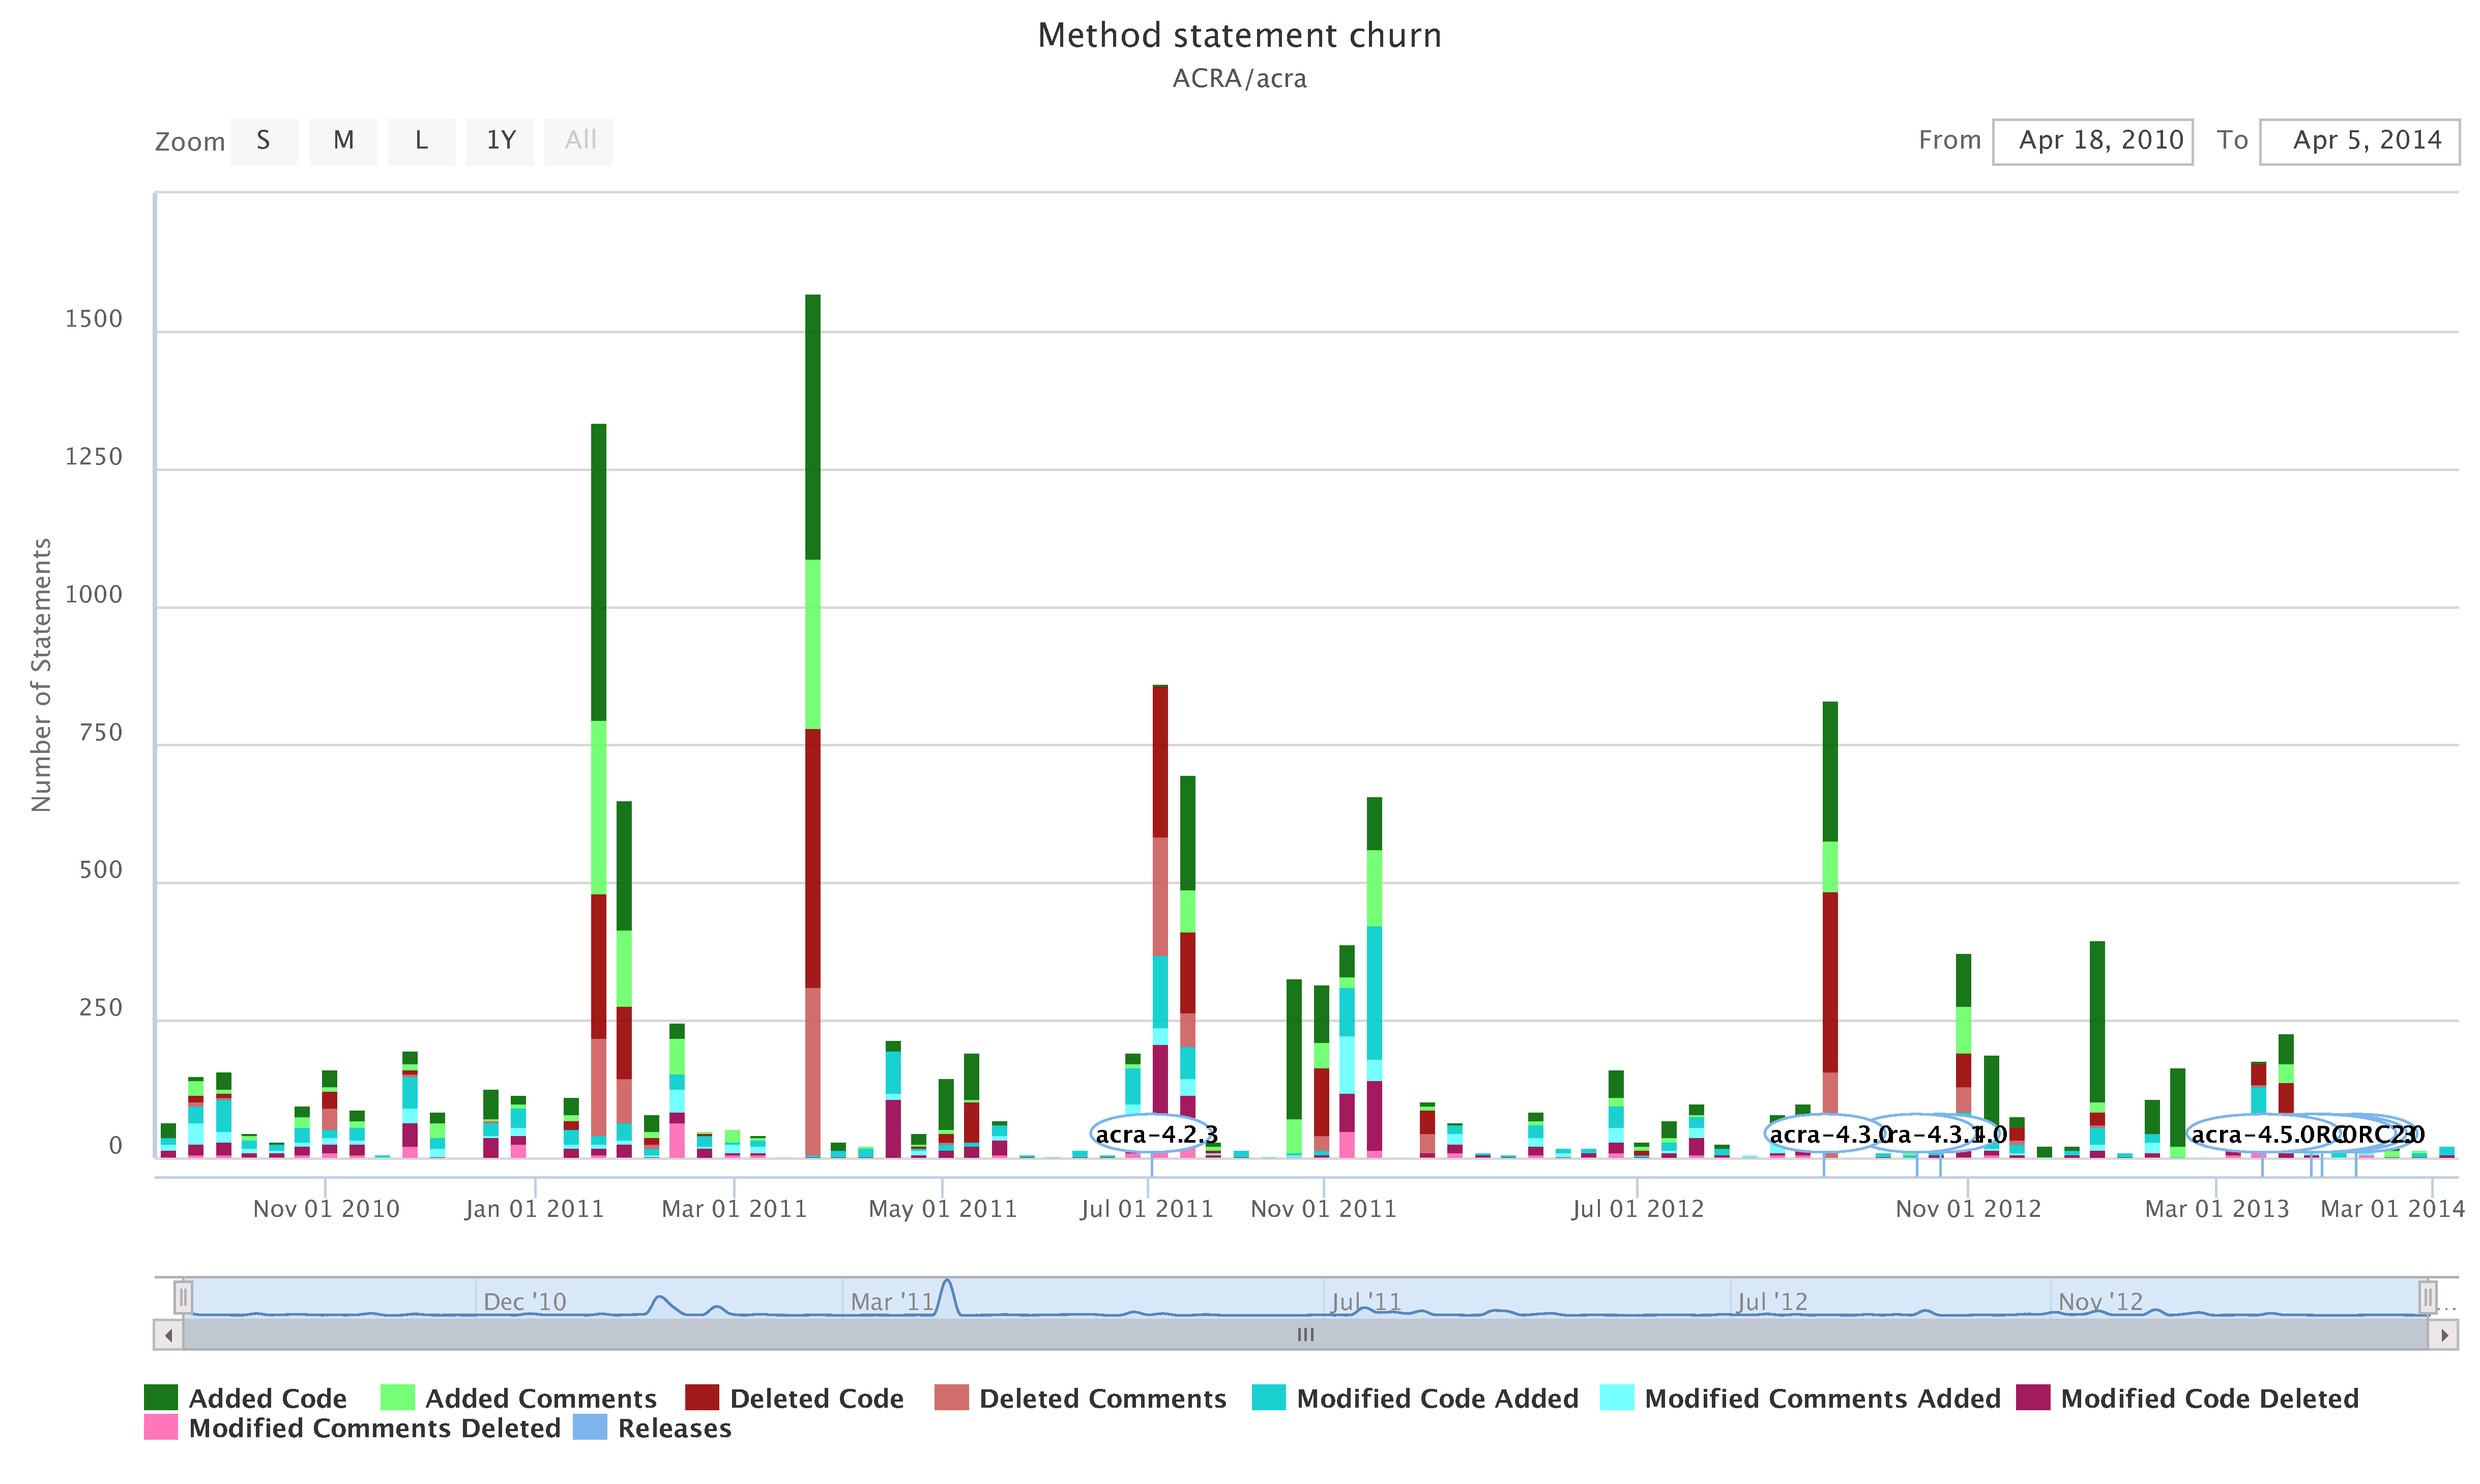
\includegraphics[width=1.0\textwidth]{images/statement_visual_acra}
%     \caption{Method Statement Change Visualization for acra}
%     \label{fig:statement_visual_acra}
% \end{figure}

% \begin{landscape}
%  \begin{figure}
%   \centering
%     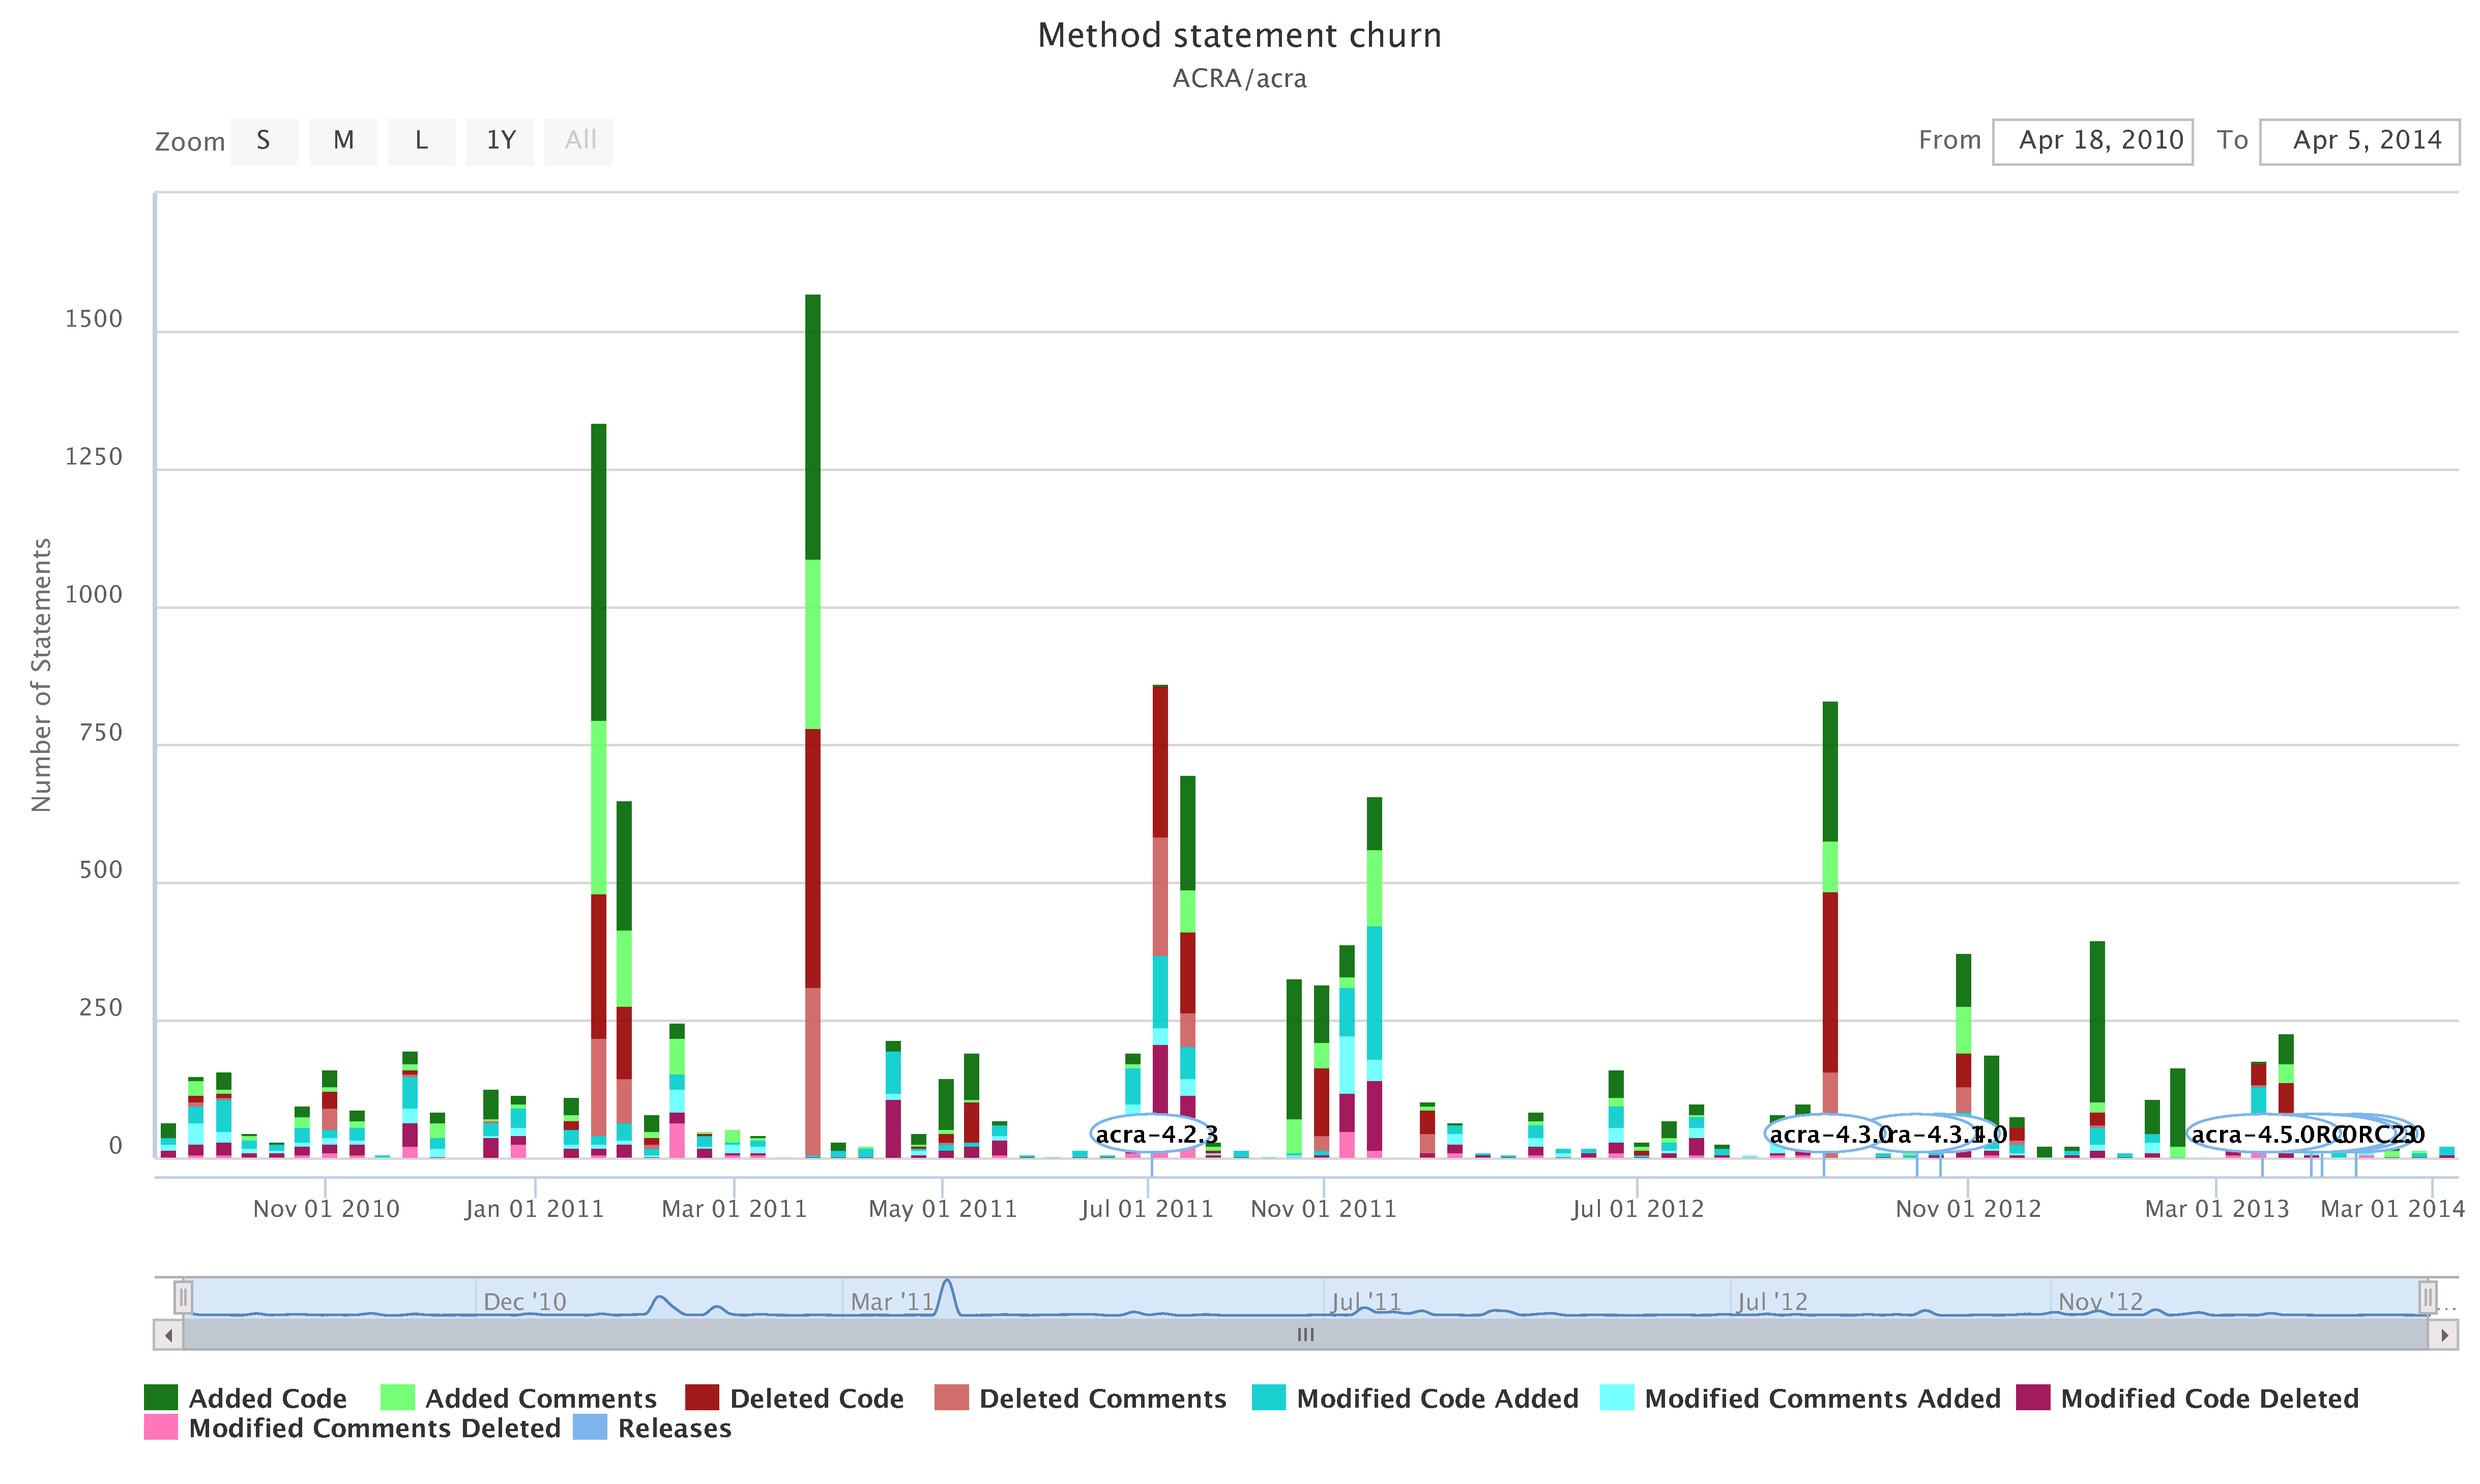
\includegraphics[width=1.5\textwidth]{images/statement_visual_acra}
%     \caption{Method Statement Change Visualization for acra}
%     \label{fig:statement_visual_acra}
%  \end{figure}
% \end{landscape}

% TODO talk about each of them specifically
\begin{landscape}
\thispagestyle{empty}
 \begin{figure}
  \centering
        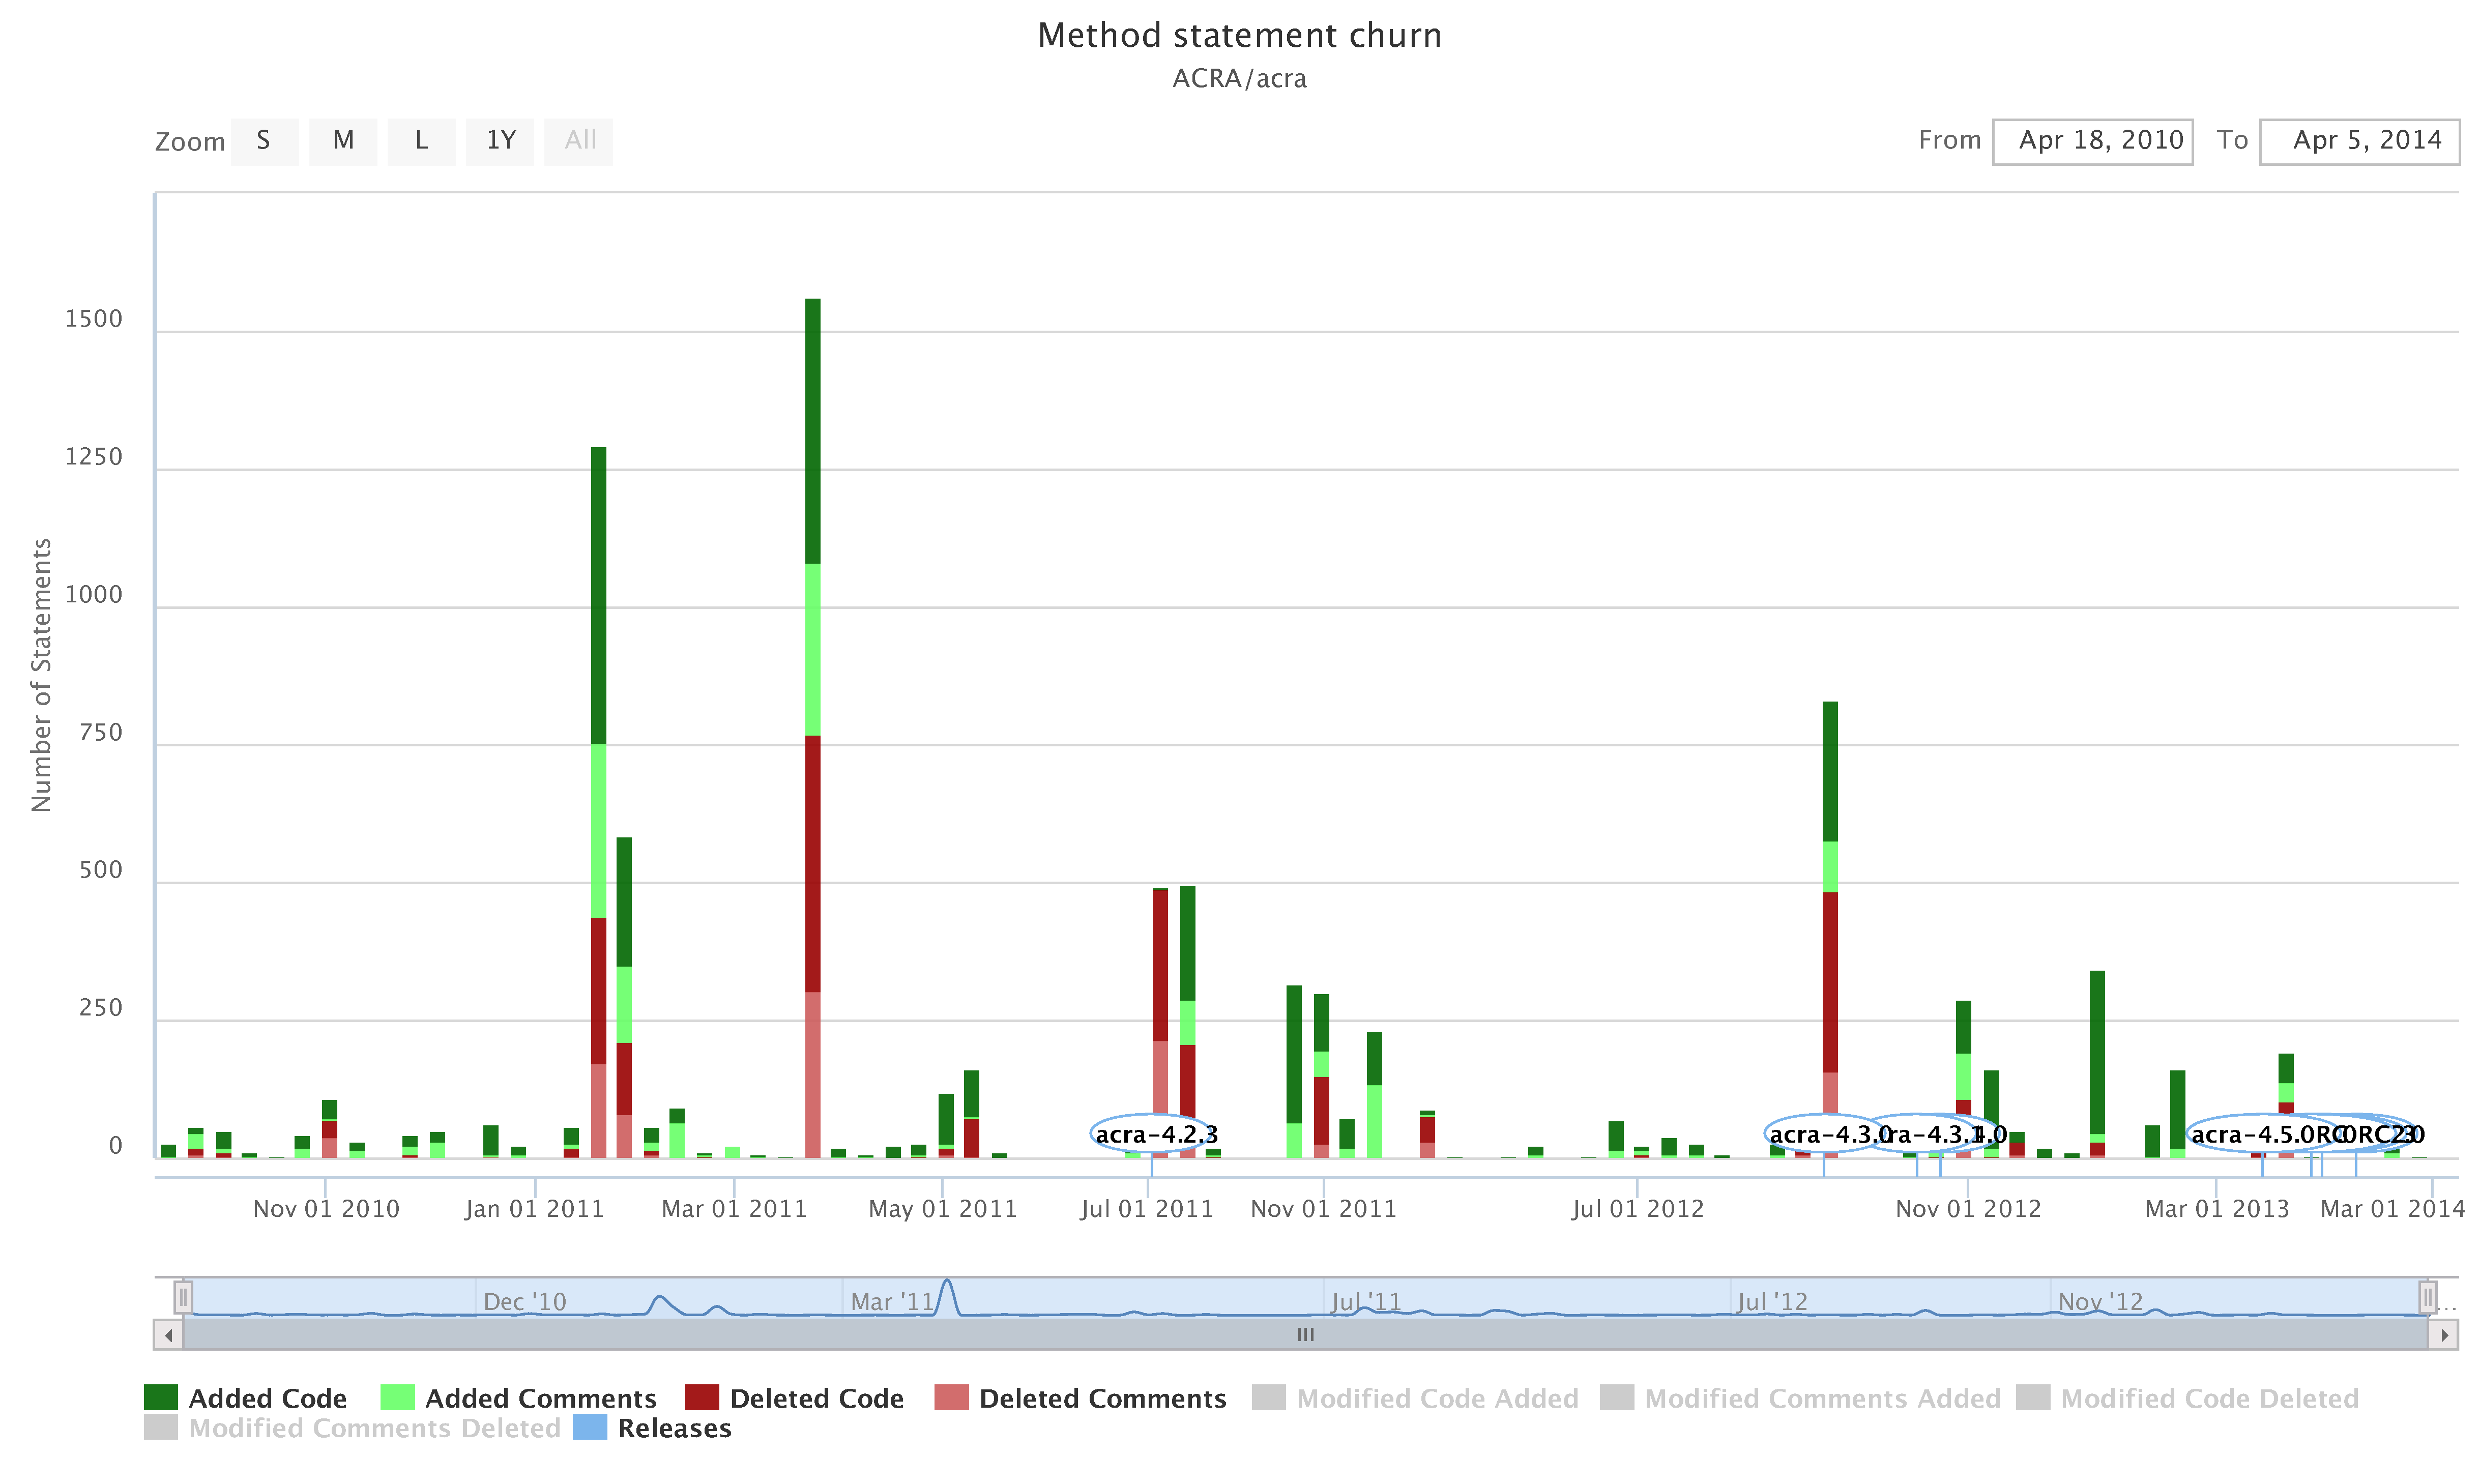
\includegraphics[width=1.5\textwidth]{images/statement_add_delete}
    \caption{Method Statement Added \& Deleted Visualization for acra}
    \label{fig:statement_add_delete_visual_acra}
 \end{figure}
\end{landscape}
\thispagestyle{plain}

\begin{landscape}
\thispagestyle{empty}
 \begin{figure}
  \centering
        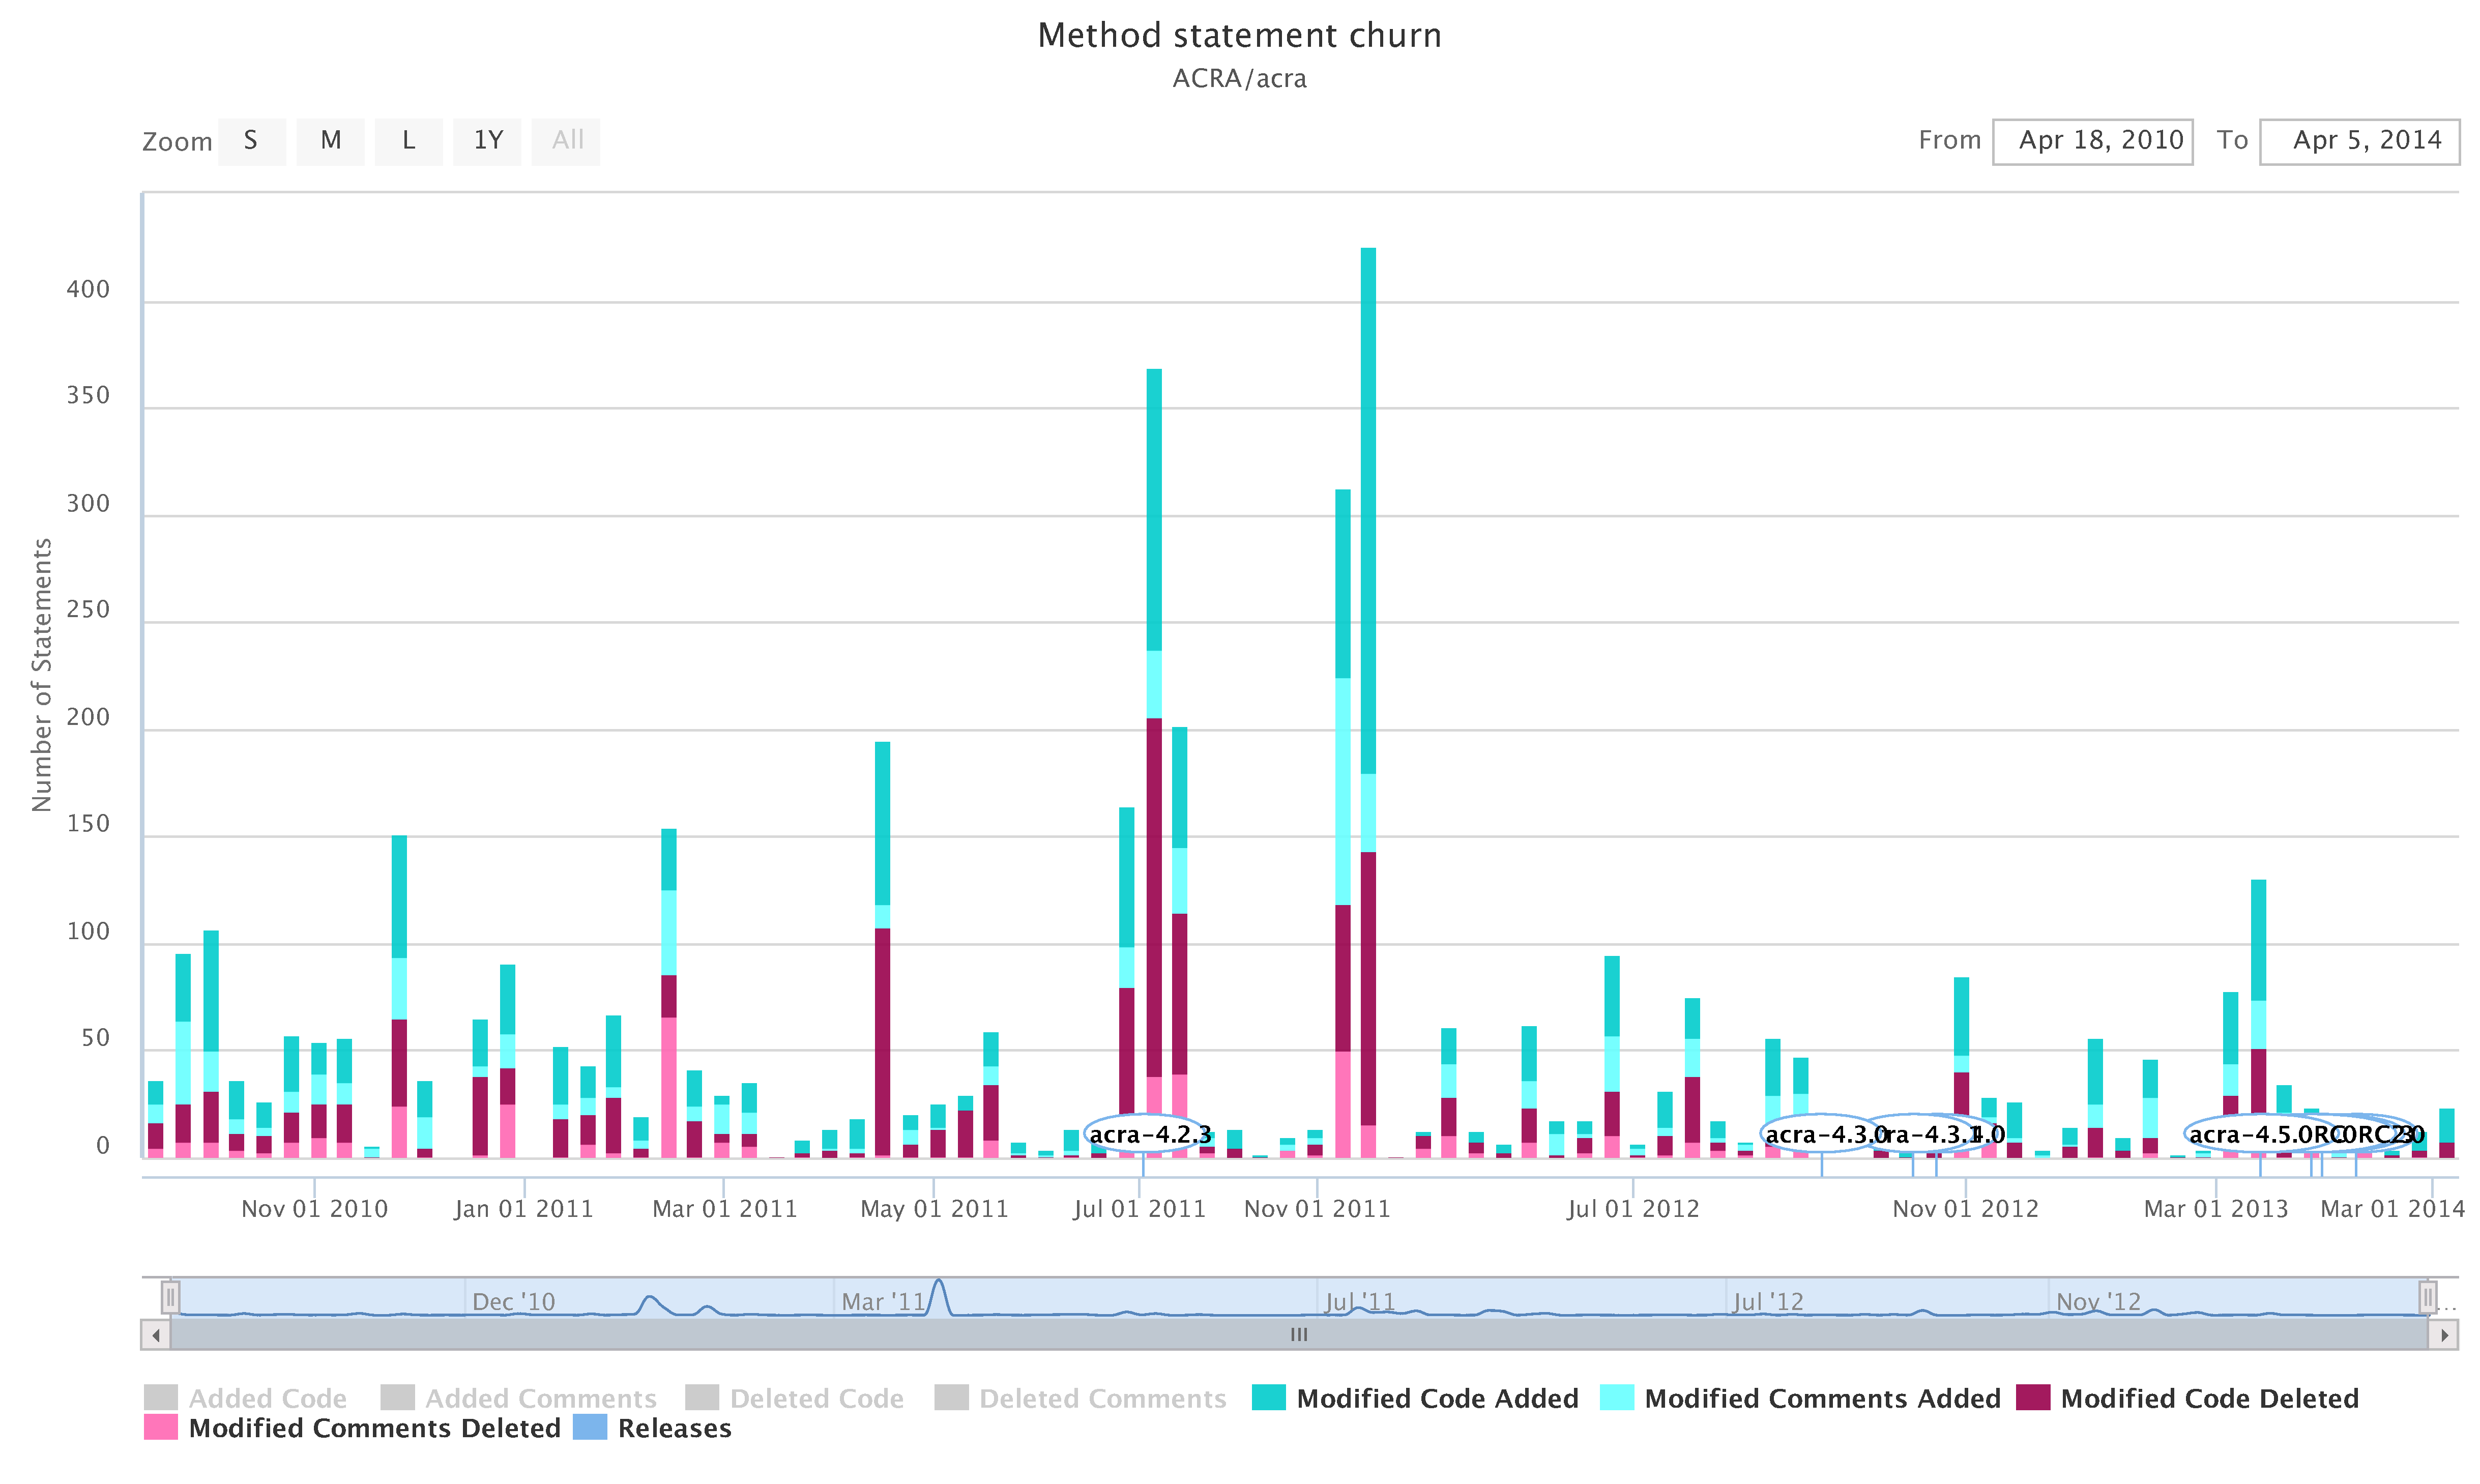
\includegraphics[width=1.5\textwidth]{images/statement_modified}
    \caption{Method Statement Modification Visualization for acra}
    \label{fig:statement_modified_visual_acra}
 \end{figure}
\end{landscape}
\thispagestyle{plain}

% Decided whether to keep the other names or update them to these ones (on the site as well).
%So finally we have the categories: \textit{Modified Code Addition}, \textit{Modified Comment Addition}, \textit{Modified Code Deletion} and \textit{Modified Comment Deletion}.